\documentclass[leqno, openany]{memoir}
\setulmarginsandblock{3.5cm}{3.5cm}{*}
\setlrmarginsandblock{3cm}{3.5cm}{*}
\checkandfixthelayout

\usepackage{amsmath}
\usepackage{amssymb}
\usepackage{amsthm}
%\usepackage{MnSymbol}
\usepackage{bm}
\usepackage{accents}
\usepackage{mathtools}
\usepackage{tikz}
\usetikzlibrary{decorations.pathmorphing,shapes}
\usetikzlibrary{calc}
\usetikzlibrary{automata,positioning}
\usepackage{tikz-cd}
\usepackage{forest}
\usepackage{braket} 
\usepackage{listings}
\usepackage{mdframed}
\usepackage{verbatim}
\usepackage{physics}
\usepackage{stmaryrd}
% \usepackage{spectralsequences} 
\usepackage{mathrsfs} 
\usepackage{stackengine} 
%\usepackage{/home/patrickl/homework/macaulay2}

%font
\usepackage[sc]{mathpazo}
\usepackage{eulervm}
\usepackage[scaled=0.86]{berasans}
\usepackage{inconsolata}
\usepackage{microtype}

%CS packages
\usepackage{algorithmicx}
\usepackage{algpseudocode}
\usepackage{algorithm}

% typeset and bib
\usepackage[english]{babel} 
\usepackage[utf8]{inputenc} 
\usepackage[T1]{fontenc}
\usepackage[backend=biber, style=alphabetic]{biblatex}
\usepackage[bookmarks, colorlinks, breaklinks]{hyperref} 
\hypersetup{linkcolor=black,citecolor=black,filecolor=black,urlcolor=black}

% other formatting packages
\usepackage{float}
\usepackage{booktabs}
\usepackage[shortlabels]{enumitem}
\usepackage{csquotes}
\usepackage{titlesec}
\usepackage{titling}
\usepackage{fancyhdr}
\usepackage{lastpage}
\usepackage{parskip}
\usepackage{graphicx}
\graphicspath{{./images/}}

\usepackage{lipsum}

% delimiters
\DeclarePairedDelimiter{\gen}{\langle}{\rangle}
\DeclarePairedDelimiter{\floor}{\lfloor}{\rfloor}
\DeclarePairedDelimiter{\ceil}{\lceil}{\rceil}


\newtheorem{thm}{Theorem}[section]
\newtheorem{cor}[thm]{Corollary}
\newtheorem{prop}[thm]{Proposition}
\newtheorem{lem}[thm]{Lemma}
\newtheorem{conj}[thm]{Conjecture}
\newtheorem{quest}[thm]{Question}

\theoremstyle{definition}
\newtheorem{defn}[thm]{Definition}
\newtheorem{defns}[thm]{Definitions}
\newtheorem{con}[thm]{Construction}
\newtheorem{exm}[thm]{Example}
\newtheorem{exms}[thm]{Examples}
\newtheorem{notn}[thm]{Notation}
\newtheorem{notns}[thm]{Notations}
\newtheorem{addm}[thm]{Addendum}
\newtheorem{exer}[thm]{Exercise}

\theoremstyle{remark}
\newtheorem{rmk}[thm]{Remark}
\newtheorem{rmks}[thm]{Remarks}
\newtheorem{warn}[thm]{Warning}
\newtheorem{sch}[thm]{Scholium}

% unnumbered theorems
\theoremstyle{plain}
\newtheorem*{thm*}{Theorem}
\newtheorem*{prop*}{Proposition}
\newtheorem*{lem*}{Lemma}
\newtheorem*{cor*}{Corollary}
\newtheorem*{conj*}{Conjecture}

% unnumbered definitions
\theoremstyle{definition}
\newtheorem*{defn*}{Definition}
\newtheorem*{exer*}{Exercise}
\newtheorem*{defns*}{Definitions}
\newtheorem*{con*}{Construction}
\newtheorem*{exm*}{Example}
\newtheorem*{exms*}{Examples}
\newtheorem*{notn*}{Notation}
\newtheorem*{notns*}{Notations}
\newtheorem*{addm*}{Addendum}

\theoremstyle{remark}
\newtheorem*{rmk*}{Remark}

% shortcuts
\newcommand{\Ima}{\mathrm{Im}}
\newcommand{\A}{\mathbb{A}}
\newcommand{\G}{\mathbb{G}}
\newcommand{\N}{\mathbb{N}}
\newcommand{\R}{\mathbb{R}}
\newcommand{\C}{\mathbb{C}}
\newcommand{\Z}{\mathbb{Z}}
\newcommand{\Q}{\mathbb{Q}}
\renewcommand{\k}{\Bbbk}
\renewcommand{\P}{\mathbb{P}}
\newcommand{\M}{\overline{M}}
\newcommand{\g}{\mathfrak{g}}
\newcommand{\h}{\mathfrak{h}}
\newcommand{\n}{\mathfrak{n}}
\renewcommand{\b}{\mathfrak{b}}
\newcommand{\ep}{\varepsilon}
\newcommand*{\dt}[1]{%
   \accentset{\mbox{\Huge\bfseries .}}{#1}}
\renewcommand{\abstractname}{Official Description}
\newcommand{\mc}[1]{\mathcal{#1}}
\newcommand{\T}{\mathbb{T}}
\newcommand{\mf}[1]{\mathfrak{#1}}
\newcommand{\mr}[1]{\mathrm{#1}}
\newcommand{\ms}[1]{\mathsf{#1}}
\newcommand{\ol}[1]{\overline{#1}}
\newcommand{\on}[1]{\operatorname{#1}}
\newcommand{\ul}[1]{\underline{#1}}
\newcommand{\wt}[1]{\widetilde{#1}}
\newcommand{\wh}[1]{\widehat{#1}}
\renewcommand{\div}{\operatorname{div}}
\newcommand{\Sm}{\mathsf{Sm}}
\newcommand{\Cor}{\mathsf{Cor}}
\newcommand{\1}{\mathbf{1}}
\newcommand{\2}{\mathbf{2}}
\newcommand{\3}{\mathbf{3}}
\newcommand{\I}{\mathrm{I}}
\newcommand{\II}{\mr{I}\hspace{-1.3pt}\mr{I}}
\newcommand{\III}{\mr{I}\hspace{-1.3pt}\mr{I}\hspace{-1.3pt}\mr{I}}
\newcommand{\ateb}{\reflectbox{$\beta$}}

\DeclareMathOperator{\Der}{Der}
\DeclareMathOperator{\Hom}{Hom}
\DeclareMathOperator{\End}{End}
\DeclareMathOperator{\ad}{ad}
\DeclareMathOperator{\Ad}{Ad}
\DeclareMathOperator{\Aut}{Aut}
\DeclareMathOperator{\Rad}{Rad}
\DeclareMathOperator{\Pic}{Pic}
\DeclareMathOperator{\supp}{supp}
\DeclareMathOperator{\Supp}{Supp}
\DeclareMathOperator{\sgn}{sgn}
\DeclareMathOperator{\spec}{Spec}
\DeclareMathOperator{\rk}{rk}
\DeclareMathOperator{\Spec}{Spec}
\DeclareMathOperator{\proj}{Proj}
\DeclareMathOperator{\Proj}{Proj}
\DeclareMathOperator{\ord}{ord}
\DeclareMathOperator{\Div}{Div}
\DeclareMathOperator{\Bl}{Bl}
\DeclareMathOperator{\ch}{ch}
\DeclareMathOperator{\td}{td}
\DeclareMathOperator{\Tor}{Tor}
\DeclareMathOperator{\depth}{depth}
\DeclareMathOperator{\CH}{CH}
\DeclareMathOperator{\Ob}{Ob}
\DeclareMathOperator{\Rat}{Rat} 
\DeclareMathOperator{\coker}{coker}
\DeclareMathOperator{\Hilb}{Hilb}
\DeclareMathOperator{\Sym}{Sym}
\DeclareMathOperator{\Ext}{Ext}

% Section formatting
\titleformat{\section}
    {\Large\sffamily\scshape\bfseries}{\thesection}{1em}{}
\titleformat{\subsection}[runin]
    {\large\sffamily\bfseries}{\thesubsection}{1em}{}
\titleformat{\subsubsection}[runin]{\normalfont\itshape}{\thesubsubsection}{1em}{}

\title{COURSE TITLE}
\author{Lectures by INSTRUCTOR, Notes by NOTETAKER}
\date{SEMESTER}

\newcommand*{\titleSW}
    {\begingroup% Story of Writing
    \raggedleft
    \vspace*{\baselineskip}
    {\Huge\itshape DAHA and Knot Homology Learning Seminar \\ Fall 2021}\\[\baselineskip]
    {\large\itshape Notes by Patrick Lei}\\[0.2\textheight]
    {\Large Lectures by Various}\par
    \vfill
    {\Large \sffamily Columbia University}
    \vspace*{\baselineskip}
\endgroup}
\pagestyle{simple}

\chapterstyle{ell}

%\renewcommand{\cftchapterpagefont}{}
\renewcommand\cftchapterfont{\sffamily}
\renewcommand\cftsectionfont{\scshape}
\renewcommand*{\cftchapterleader}{}
\renewcommand*{\cftsectionleader}{}
\renewcommand*{\cftsubsectionleader}{}
\renewcommand*{\cftchapterformatpnum}[1]{~\textbullet~#1}
\renewcommand*{\cftsectionformatpnum}[1]{~\textbullet~#1}
\renewcommand*{\cftsubsectionformatpnum}[1]{~\textbullet~#1}
\renewcommand{\cftchapterafterpnum}{\cftparfillskip}
\renewcommand{\cftsectionafterpnum}{\cftparfillskip}
\renewcommand{\cftsubsectionafterpnum}{\cftparfillskip}
\setrmarg{3.55em plus 1fil}
\setsecnumdepth{subsection}
\maxsecnumdepth{subsection}
\settocdepth{subsection}

\begin{document}
    
\begin{titlingpage}
\titleSW
\end{titlingpage}

\thispagestyle{empty}
\section*{Disclaimer}%
\label{sec:disclaimer}

These notes were taken during the seminar using the \texttt{vimtex} package of
the editor \texttt{neovim}.  Any errors are mine and not the speakers'.  In
addition, my notes are picture-free (but will include commutative diagrams) and
are a mix of my mathematical style and that of the lecturers.  If you find any
errors, please contact me at \texttt{plei@math.columbia.edu}.

I patched the notes from \'Alvaro's lecture using his notes, which contain some
material not covered during the lecture. The notes here only contain material
covered during the lecture.

\vspace*{1cm}

\noindent\textbf{Seminar Website:}\\
\url{https://math.columbia.edu/~samdehority/seminars/2021-fall-seminar-knot-homology} \newpage

\tableofcontents

\chapter{Sebastian (Sep 14): Khovanov Homology}%
\label{cha:sebastian_sep_14_khovanov_homology}

Recall that the \textit{Kauffman bracket} of a link diagram $D$ has axioms $\ev{\emptyset} = 1$, $\ev{0 \sqcup D} = (q+q^{-1}) \ev{D}$, and for any crossing
\[ \ev{\text{crossing}} = q \ev{\text{horizontal}} + q^{-1} \ev{\text{vertical}} \]
If $D$ has $n_+$ positive crossings and $n_-$ negative crossings, then the \textit{Jones polynomial} of the underlying link $L$ is $J(L) = {(-1)}^n q^{n_+ - 2n_-} \ev{D}$.

We may have heard that Khovanov homology is a categorification of the Jones polynomial. To motivate this, there are quantum invariants like the Jones polynomial, the HOMFLY polynomial, WRT, and others. On the other side, there are gauge-theoretic invariants like instanton Floer homology and the Casson invariant. The quantum invariants generally come from representations of quantum groups are are combinatorial, but it is unclear what geometric information we obtain. On the other hand, the gauge theoretic invariants are more powerful, but of course harder to compute. We want to consider relations between the two types of invariants.

Some of the gauge-theoretic invariants end up being Euler characteristics; for example, the Casson invariant is twice the Euler characteristic of instanton Floer homology.

For a link diagram $L$, we will introduce a bigraded $\Z$-module $\mr{ Kh }^{*,*}(L)$ such that 
\[ J(L) = \sum_{i,j} {(-1)}^i q^j \rk_{\Z} \mr{ Kh }^{i,j}(L). \]

\section{Category of Pictures}%
\label{sec:category_of_pictures}

Given $D$, we will order its crossings. For each crossing we have a $0$-resolution (horizontal) and a $1$-resolution (vertical). If $n = n_+ + n_-$, then each element of $\qty{0,1}^n$ gets a complete resolution, which is a collection of circles in the plane. For example, consider the Hopf link with resolution. 

% insert picture here
\begin{figure}[H]
    \centering
    \includegraphics[width=0.8\linewidth]{seb1.png}
    \caption{Hopf link and resolution}%
    \label{fig:seb1}
\end{figure}

Then we have
\[ \ev{H} = {(q+q^{-1})}^2 - q(q+q^{-1}) - q(q+q^{-1}) + q^2 (q+q^{-1}) = q^4 + q^2 + 1 + q^{-2}, \]
and thus 
\[ J(H) = {(-1)}^2 q^{-4} \ev{H} = 1 + q^{-2} + q^{-4} + q^{-6}. \]
Changing a $0$-resolution to a $1$-resolution is given by a saddle, or a cobordism.

Let $\ol{\ms{Cob}^3}$ be the category with objects collections of oriented circles in $\R^2$ and morphisms oriented cobordisms in $\R^2 \times [0,1]$. For each $\Sigma \in \Hom(O_1, O_2)$, we define $\deg \Sigma = \chi(\Sigma)$. Then we add objects $O\qty{m}$ for each $O \in \mr{Obj}(\ol{\ms{Cob}^3})$ and $m \in \Z$. This gives a graded category $\ms{Cob}^3$. Now let $\ms{Mat}(\ms{Cob}^3)$ denote the additive closure of $\ms{Cob}^3$ and $\ms{Kom}(\ms{Mat}(\ms{Cob}^3))$ be its category of chain complexes.

Now for each $\alpha \in \qty{0,1}^n$, we assign the object $O\qty{m}$, where $O$ is the resolution of $L$ obtained from the $\alpha_i$-resolution at the $i$-th crossing and $m = \sum \alpha_i$. For each edge, we will assign the saddle cobordism between objects at each edge.

\begin{figure}[H]
    \centering
    \includegraphics[width=0.8\linewidth]{seb3.png}
    \caption{Saddle cobordism}%
    \label{fig:seb2}
\end{figure}

To obtain $d^2 = 0$, we need that all square faces in the diagram anti-commute. The problem is that in the diagram, the two cobordisms are actually the same (we can reorder the saddles), so now we need to add signs to the edges such that each square face has an odd numbder of minus signs. In the example of the Hopf link, we just add a minus sign to the $10 \to 11$ edge.

Now we may construct the $m$-th chain group ${ [[L]] }^m$ of $[[L]]$ to be
\[ \bigoplus_{\alpha \mid \sum \alpha_i = m} (\text{resolution over $\alpha$}). \]
The chain homotopy type of $[[L]]$ is a link invariant after passing to a quotient $\ms{Cob}^3/\ell$ of $\ms{Cob}^3$ by the following relations:

\begin{figure}[H]
    \centering
    \includegraphics[width=0.8\linewidth]{seb5.png}
    \caption{Relations for $\ms{Cob}^3//\ell$}%
    \label{fig:seb3}
\end{figure}

Now we define the \textit{Bar-Natan category} $\ms{BN} \coloneqq \ms{Kom}(\ms{Mat}(\ms{Cob}^3/\ell))$. Of course, we now need to prove invariance under the Reidemeister moves. For the first Reidemeister move, we have the following diagram:

\begin{figure}[H]
    \centering
    \includegraphics[width=0.6\linewidth]{seb6.png}
    \caption{Diagram for R1}%
    \label{fig:seb4}
\end{figure}

Then here hare the easy relations.

\begin{figure}[H]
    \centering
    \includegraphics[width=0.8\linewidth]{seb7.png}
    \caption{Easy relations}%
    \label{fig:seb5}
\end{figure}

Finally, here we see that we have a homotopy:

\begin{figure}[H]
    \centering
    \includegraphics[width=0.8\linewidth]{seb8.png}
    \caption{The homotopy really is a homotopy}%
    \label{fig:seb6}
\end{figure}

The proofs of invariance under the other Reidemeister moves are similar, but significantly more complicated. But now any functor from $\ms{Cob}^3/\ell$ to any abelian category will give us a knot invariant. Note that such a functor does not have to be a $2$-dimensional TQFT.

\section{Khovanov Homology}%
\label{sec:khovanov_homology}

Returning to something more concrete, any cobordism in $\ms{Cob}^3/\ell$ can be decomposed into pairs of pants and caps and cups, so to specify a functor, we only need to specify what it does to four morphisms. Here, the cobordisms correspond to
\[ m \colon V \otimes V \to V \qquad \Delta \colon V \to V \otimes V \qquad \iota \colon V \to \Z \qquad \ep \colon V \to \Z, \]
where $V = \mc{F}(S^1)$ for $\mc{F}$ a TQFT. Then Khovanov homology is the functor where $V = \Z \qty{-1} \oplus \Z \qty{1}$, where $m$ is given by
\[ v_- \otimes v_- \mapsto 0 \qquad v_- \otimes v_+ \mapsto v_- \qquad v_+ \otimes v_+ \mapsto v_+ \qquad v_+ \otimes v_- \mapsto v_- ,\]
$\Delta$ is given by
\[ v_- \mapsto v_- \otimes v_- \qquad v_+ \mapsto v_+ \otimes v_- + v_- \otimes v_+, \]
$\iota$ is given by $1 \mapsto v_+$, and $\ep$ is given by $v_- \mapsto 1, v_+ \mapsto 0$. The grading on $V$ is called the \textit{Jones grading} because it records power of $q$ in the Jones polynomial.

Now we are finally able to define the Khovanov homology
\[ \mr{Kh}(L) \coloneqq H^*(\mc{F}([[L]]))[-n_-]\qty{n_+ - 2n_-} \]

\begin{thm}
    We have the formula
    \[ J(L) = \sum_{i,j} {(-1)}^i q^j \rk_{\Z} \mr{ Kh }^{i,j}(L). \]
\end{thm}

For the Hopf link, the chain complex is given by
\[ (V \otimes V)\qty{-4} \xrightarrow{m \oplus m} V \qty{-3} \oplus V\qty{-3} \xrightarrow{\Delta^1 - \Delta^2} (V \otimes V) \qty{-2}, \]
and thus we can compute the Khovanov homology.

\begin{thm}[Jacobsson, Bar-Natan]
    The map on $[[L]]$ associated to a cobordism in $\R^3 \times [0,1]$ is independent of its decomposition into elementary cobordisms up to a sign and cobordisms in the Bar-Natan category.
\end{thm}

\chapter{\'Alvaro (Sep 21): HOMFLY-PT homology}%
\label{cha:'alvaro_sep_21_homfly_pt_homology}

If we already know about Hecke algebras, then we could discover the HOMFLY-PT polynomial with the unknot being $1$ and the skein relation
\[ t \cdot \text{under} + t^{-1} \cdot \text{over} = z \cdot \text{unlinked}. \]
Here, if we set $t = q^{2N}$ and $z = q + q^{-1}$, we recover the $SL_2$ link polynomial and if we set $N = 1$, we recover the Jones polynomial.

The reason that we could have discovered the HOMFLY-PT polynomial is using the representation theory of the braid group, which is generated by $s_1, \ldots, s_{n-1}$ with relations $s_i s_{i+1} s_i = s_{i+1} s_i s_{i+1}$ and $s_i s_j = s_j s_i$ if $\abs{i-j} \geq 2$.

First, note that every link is the closure of a braid. Then two braids give rise to isotopic links if they are related by Markov moves. Now we consider
\[ \Z[q^{\pm}] \mr{Br}_n \twoheadrightarrow H(S_n) = \Z[q^{\pm}] \cdot \qty{\delta_w \mid w \in S_n} / \delta_s^2 = \delta_s (q-1) + q. \]
Now we can define a trace map
\[ \Tr \colon \bigcup_{n \geq 1} H(S_n) \to \Z[q^{\pm}, z^{\pm}] \]
with the condition that $\Tr(x s_n y) = z \Tr(xy)$ and $\Tr(1) = 1$. In particular, these imply that $\Tr(xy) = \Tr(yx)$, and this is called the \textit{Oceanu trace}. If we normalize the $s_i$, then $\Tr(x s_i) = \Tr(x s_i^{-1})$. Then under the correct normalization, we obtain the HOMFLY-PT polynomial.

\section{Triply graded homology}%
\label{sec:triply_graded_homology}

This was discovered by Khovanov-Rozansky in 2004 using matrix factorizations and Khovanov in 2005 using Soergel bimodules. Then work of various subsets of Elias, Hogancamp, and Mellit computed HHH for torus $(m,n)$-links.

Consider the symmetric group $S_m = \ev{s_1, \ldots, s_{m-1}}$. Then consider $R = \Q[x_1, \ldots, x_m]$, where the $x_i$ have degree $2$. Then we have a natural action of $S_m$ on $R$, and $R^{S_i}$ are the invariants. Then we will define $B_{s_i} = R \otimes_{R^s} R(1)$ as an $R$-bimodule, and for $\ul{w} = s_{i_1} \cdots s_{i_n}$, we will define the \textit{Bott-Samuelson bimodule} $BS(\ul{w}) = B_{s_{i_1}} \otimes \cdots \otimes B_{s_{i_n}}$. Next, if we consider the Bott-Samuelson bimodules and add in all tensor products and direct sums, we obtain the Hecke category $\ms{SBim}$, which categorifies the Hecke algebra.

In our running example, we will take $S_2 = \qty{1, s}$ and $R = \Q[x_1, x_2]$. Here, we will take $R^s = \Q[x_1+x_2, (x_1-x_2)^2]$, and we will write $r = x_1+x_2, t = x_1-x_2$. Therefore, we have
\[ BS(s^2) = B_s \otimes_R B_s = R \otimes_{R^s} R \otimes_R R \otimes_{R^s} R(2) = R \otimes_{R^s} R \otimes_{R^s} R(2). \]

\begin{thm}[Soergel's categorification theorem]
    Note that $H(S_n)$ has a KL-basis $\qty{b_w \mid w \in S_n}$. Then there is a bijection between indecomposables in $\ms{SBim}$ and the KL-basis taking the tensor product to multiplication.
\end{thm}

Now if we write $b_{s_i} = \delta_{s_i} + q$, we have $b_{s_i}^2 = q b_{s_i} + q^{-1} b_{s_i}$. On the other side, we have
\begin{align*}
    B_s^{\otimes 2} &= R \otimes_{R^2} \otimes R \otimes R(2) \\
    &= R \otimes (\Q[r,t^2] \oplus t \Q[r,t^2]) \otimes_{R^2} R(2) \\
    &= R \otimes_{R^s} R(2) \oplus R \otimes_{R^s} R \\
    &= B_s(1) \oplus B_s(-1).
\end{align*}

Now we will categorify the braid group and construct HHH. We have $b_s = \delta_s + q$ and thus $\delta_s = b_s - q$, so in the categorified version we will have $q_i \colon B_{s_i} \to R$. Then we consider the complex
\[ F_{s_i} = 0 \to \ul{B_{s_i}} \xrightarrow{q_i} R(1) \to 0 \to \cdots \]
and analogously
\[ F_{s_i}^{-1} = R(-1) \xrightarrow{d_i} \ul{B_{s_i}} \to 0 \to \cdots \]

\begin{thm}[Rouquier]
    The assignment $\ul{w} \to F^{\bullet}(\ul{w}) = F_{s_1^{\pm}} \otimes \cdots \otimes F_{s_{i_n}^{\pm}}$ is a well-defined homomorphism $\mr{Br}_n \to K^{b}(\ms{SBim})$.
\end{thm}

Now we apply the Hochschild homology $HH_n$ to $F^{\bullet}(w)$, and we obtain the complex
\[ HH_n(F^{-1}(w)) \to HH_n(F^0(w)) \to HH_n(F^1(w)), \]
and taking the homology, we obtain the HHH homology. The grading is given by the homological grading $HH_i(F^j(\ul{w}))$ that modifies $j$, the Hochschild grading, and the internal grading as $R$-graded bimodules.

\section{Hochschild homology}%
\label{sec:hochschild_homology}

Next we observe that Hochschild homology is easier for polynomial rings. Recall that if $R$ is a $k$-algebra, then if we write $R^{env} = R \otimes_k R^{op}$, we have
\[ HH_n(-) = \Tor_n^{R^{env}}(R,-). \]
Instead of the bar complex, we will consider the Koszul complex
\[ K^{\bullet} \bigwedge^n V \otimes R^{env} \to \cdots \to V \otimes R^{env} \to R^{env} \to R \to 0, \]
which is a free resolution of $R$, where $V = \Q^m$. Then this complex computes the Hochschild homology. For example, if $R = \Q[x] = M$ where $\deg x = 2$, we have
\[ K^{\bullet} = R^{env}(-2) \xrightarrow{(x \otimes 1 - 1 \otimes x)} R^{env} \] and $R(-2) \xrightarrow{0} R$, and thus
\[ HH_*(R) = \begin{cases}
    \Q[x] & * = 0 \\ 
    \Q[x](-2) & * = 1.
\end{cases}
\]

for another example, when $R = \Q[x,y]$ and $M$ is a graded $R$-bimodule, and $\deg x = \deg y \ 2$, we have
\[ K^{\bullet} = R^{env}(-4) \to R^{env}(-2) \oplus R^{env}(-2) \to R^{env} \]
where the maps are given by $(x \otimes 1 - 1 \otimes x, 1 \otimes y - y \otimes 1)$ and $(y \otimes 1 - 1 \otimes y, x \otimes 1 - 1 \otimes x)$, and the Koszul resolution of $M$ is similar.

\section{Example of triply graded homology}%
\label{sec:example_of_triply_graded_homology}

Now the unknot is the closure of $1 \in \mr{Br}_1$, and so we want to compute its homology $HHH_{***}$. We know that
\[ F^{\bullet}(1) = 0 \to \ul{R} \to 0, \]
and therefore
\[ HH_*(R) = \begin{cases}
    \Q[x] & * = 0 \\ 
    \Q[x](-2) & * = 1.
\end{cases}
\]
The Euler characteristic is
\[ (1 + q^2 + q^4 + \cdots) + a (q^2 + q^4 + \cdots) = \frac{1+aq^2}{1-q^2}, \]
and this recovers the unknot.

Now if we take the closure of $s \in \mr{Br}_2$, which is still the unknot, we have
\[ F^{\bullet}(S) = \ul{B_s} \to R(1) ,\]
where $R = \Q[x_1, x_2]$. But now we need to compute the Hochschild homology
\[ HH_*(B_s) \to HH_*(R(1)) \]
in all degrees. For $R(1)$, the Koszul resolution is
\[ R(-3) \xrightarrow{0} { R(-1) }^{\oplus 2} \xrightarrow{0} R(-1) \]
and for $B_s$ it is
\[ B_s(-4) \xrightarrow{(f,f)} B_s(-2) \oplus B_s(-2) \xrightarrow{(-f,f)} B_s, \]
where $R^s = \Q[s,t^2]$ and $f(m) = \frac{1}{2} tm - \frac{1}{2} mt$. Now we have $\ker(f) = \ev{mt+tm}, \Im(f) = mt-tm$. Now we compute $HH_0(B_s) = B_s/\Im f$, $HH_*(B_s) = R(-1) \oplus \ker(f)(-2)$, and $HH_2(B_s) = \ker(f)(-4)$. Then the three maps are the identity in degree $0$, $(\mr{id}, i)$ in degree $1$, and $i$ in degree $2$, where $i$ is the counit. Finally we obtain the following table for the HHH:
\begin{table}[H]
    \centering
    \caption{HHH homology}
    \label{tab:label}
    \begin{tabular}{ccc}
    \toprule
    Hochschild degree & $HHH_{0**}(s_1)$ & $HHH_{1**}(s_1)$ \\
    \midrule
        $0$ & $0$ & $0$ \\
        $1$ & $0$ & $\Q[r](-1)$ \\
        $2$ & $0$ & $\Q[r](-3)$
    \end{tabular}
\end{table}

This is isomorphic to $HHH(1)$ in the previous example after a shift.

Finally consider the Hopf link, which is the closure of $s^2$. Here $F^{\bullet}(s^2)$ is given by
\begin{equation*}
\begin{tikzcd}
    B_s^{\otimes 2} \ar{r} \ar{d} & B_s(-1) \ar{d} \\
    B_s(1) \ar{r} & R(2).
\end{tikzcd}
\end{equation*}
This complex is homotopic to $B_s(-1) \to B_s(1) \to R(2)$.

\section{Connections to geometry}%
\label{sec:connections_to_geometry}

Define the matrix $B_i(z)$ to have the matrix $\begin{psmallmatrix}
    0 & 1 \\ 1 & z
\end{psmallmatrix}$ in the $i$-th position. Then we have the identity
\[ B_i(z_1) B_{i+1}(z_2) B_i(z_3) = B_{i+1}(z_3) B_i(z_2 - z_1 z_3) B_{i+1}(z_1). \]
For a positive braid $\beta = s_{i_1} \cdots s_{i_n}$, we assign the matrix $B_{\beta}(z_1, \ldots, z_n) = B_{i_1}(z_1) \cdots B_{i_n}(z_n)$, and finally we consider the variety 
\[ X(\beta) = \qty{(z_1, \ldots, z_n) \in \C^n \mid B_{\beta}(z_1, \ldots, z_n) \text{ is upper triangular}}. \]
For example, if $\beta$ is the trefoil knot, then $X(\beta) = \qty{1 + z_1 z_2 = 0}$. There is a torus action on this variety, where if we have $n$ strands there is an action of ${(\C^{\times})}^{n-1}$. In this example, we have $(z_1, z_2, z_3) \mapsto (z_1 \cdot t, z_2 \cdot t^{-1}, z_3)$.

\begin{thm}[Trinh, 2021]
    We have $H_{*,BM}^T(X(\beta))$ has a nontrivial weight filtration whose associated graded module is isomorphic to $HHH_{0**}(\beta)$.
\end{thm}

For the trefoil knot, we obtain a grading on $H_*(S^1)$.

Finally, relating this to Hilbert schemes we have the Oblomkov-Shende conjecture, where if $C$ is an integral plane curve and $p$ is a singularity, then
\[ \mr{HOMFLY}(\mr{link}(p)) = {\qty(\frac{a}{q})}^{\mu - 1} \sum_{\ell,m} q^{2\ell} {(-a^2)}^m \chi(C_p^{[\ell,\ell+m]}). \]
Next, there is the Oblomkov-Rasmussen-Shende conjecture, which says that replacing $\chi$ with $H^*$, we obtain HHH. Then there is Oblomkov-Rozansky homology, and finally a conjecture of Gorsky-Negut-Rasmussen, which says that if $X = F \mr{Hilb}_n^{dg}(\A^2)$ is a dg version of the flag Hilbert scheme, then there is a commutative diagram of monoidal functors
\begin{equation*}
\begin{tikzcd}
    K^b(\ms{SBim}_n) \ar{r}{L_*} \ar{d}{HHH} & D^b(\ms{Coh}_{\C^{\times} \times \C^{\times}}(X)) \\
    \ms{Vect}_{\Q}^{\Z^{\oplus 3}},
\end{tikzcd}
\end{equation*}
where $\ms{Vect}_{\Q}^{\Z^{\oplus 3}}$ is the category of $\Z^{\oplus 3}$-graded $\Q$-vector spaces.

\chapter{Avi (Sep 28): Hilbert Schemes}%
\label{cha:avi_sep_28_hilbert_schemes}

\section{Definitions}%
\label{sec:definitions}

Let $X$ be a projective variety over a field $k = \C$. For example, if $X = \P^n$, we in algebraic geometry are interested in projective varieties, which are closed subschemes of $X$. We are interested in classifying closed subschemes of $X$, and to do this we will construct a functor $\mr{Hilb}(X)$ given by
\[ \Hilb(X)(T) = \qty{ Z \subset T \times X \mid Z \to T \text{ flat}}. \]
We are interested in the representability of this functor, and unfortunately this functor is not representable in any reasonable way.

For example, consider $X = \P^1$. If we consider subschemes with finite support, we obtain the space
\[ \bigsqcup_n \mr{Sym}^n \P^1 = \bigsqcup_n \P^n. \]
This has infinitely many connected components and is infinite-dimensional in general. This tells us that we want to stratify our functor into pieces.

Now consider $Z \subset X = \P^n$. Then define graded coordinate ring $R = \bigoplus_i R_i$ of $Z$ and the function $i \mapsto \dim_R R_i$. For $i \gg 0$, this function equals some polynomial in $i$. More generally, let $\mc{F}$ be a quasicoherent sheaf on $X$. Then we can consider the function
\[ i \mapsto h^0(X, \mc{F}(i)), \]
and in particular, for $i \gg 0$, this function equals the Euler characteristic $\chi(\mc{F}(i))$ because for $i$ sufficiently large, all twists have vanishing higher cohomology. Finally, $\chi(\mc{F}(i))$ is a polynomial, which we will call the \textit{Hilbert polynomial} $P_{\mc{F}}(i)$.

For a subscheme $Z \subset X$ with ideal sheaf $\mc{I}_Z \subseteq \mc{O}_X$, we will define $P_Z = P_{\mc{I}_Z}$. Returning to $X = \P^1$, then if $Z$ is a scheme which is $n$ points, then $\dim H^0(X, \mc{I}_Z) = n$. For the subscheme $X$, we have $h^0(X, \mc{O}_X(i)) = i+1$. We are now able to define the functor
\[ \Hilb^f(X)(T) \coloneqq \qty{Z \subseteq T \times X \mid Z \to T \text{ flat}, P_{Z_t} = f}. \]
In particular, we have a decomposition
\[ \Hilb(X) = \bigsqcup_f \Hilb^f(X). \]
In our case, we will focus on $0$-dimensional subschemes, and we will denote both the functor and the scheme that represents it as $X^{[n]} = \Hilb^n(X)$.

\begin{exm}
    Suppose $n = 0$. All subschemes of $T \times X$ with $P_{Z_t} = 0$ must have empty fibers over $T$ and thus must be empty themselves.

    If $n = 1$, then all ideals of colength $1$ are maximal ideals, which are the same as closed points of $X$, so $X^{[1]} = X$.

    When $n = 2$, we are looking for ideals $\mc{I}$ such that $\mc{O}_X / \mc{I}$ has length $2$. Thus either this subscheme is supported at two distinct points or a single point. If the support of the subscheme is two distinct points $x_1 \neq x_2$, then at each $x_i$, the ring $\mc{O}_X/\mc{I}$ must have length $1$. Thus we have a locus $(X \times X \setminus \Delta) / S_2$. In the second case, where $\mc{O}_X / \mc{I}$ is supported at a single point $x$, then we have a sequence of inclusions
    \[ \mf{m}_x^2 \subseteq I \subset \mc{m}_X \subset \mc{O}_X. \]
    Thus we are looking for morphisms $\varphi \colon \mf{m}_x / \mf{m}_x^2 \to k$ up to a scalar, so above the point $x$ we have $\P T_{X,x}$, and therefore we have
    \[ X^{[2]} = (X \times X \setminus \Delta) / S_2 \sqcup \P T_X. \]
\end{exm}

More generally, we have a morphism $\pi \colon X^{[n]} \to \mr{Sym}^n X$ sending a subscheme $Z$ to its support $\abs{Z}$, called the \textit{Hilbert-Chow morphism}. If $\lambda = (\lambda_1, \ldots, \lambda_r)$ is a partition of $n$, we have a stratum $\Sym^{\lambda} X$ with fixed multiplicities given by $\lambda$. Thus we have
\[ \Sym^n X = \bigsqcup_{\lambda} \Sym^{\lambda} X, \]
which induces a stratification of $X^{[n]}$ into pieces $X_{\lambda}^{[n]}$.

For example, when $\lambda = (n)$, we have the Hilbert-Chow morphism
\[ X_{(n)}^{[n]} \xrightarrow{\pi} \Sym^{(n)} X = X, \]
and so the fibers are schemes $X_p^{[n]}$ parameterizing length $n$ subschemes of $X$ supported at $p$.

\begin{exm}
    When $X$ is a smooth curve, $\pi$ is actually an isomorphism. This is because all local rings $\mc{O}_{X,p}$ are discrete valuation rings, and in particular they have a unique idea of length $n$. Therefore all fibers of $\pi$ must be points.
\end{exm}

When $X$ is a smooth surface, then $X^{[n]}$ is always smooth, but in fact Hilbert schemes of points are highly singular for $n > 2$ in higher dimension.

\section{Hilbert schemes of smooth surfaces}%
\label{sec:hilbert_schemes_of_smooth_surfaces}

Now suppose that $X$ is a smooth surface. Suppose that $Z \subseteq X$ is supported at a point $p$ with length $n$. In particular, we have a chain of inclusions
\[ \mf{m}_x^n \subseteq I \subseteq \mf{m}_x^{n-1} \subset \mc{O}_{X,x}, \]
and thus this data is equivalent to $I / \mf{m}_x^n \subset \mc{O}_{X,x} / \mf{m}_x^{n-1}$. Up to completion, all of this data is independent of both $X$ and $x$, and in fact
\[ \wh{\mc{O}}_{X,x} = k[[T_1, T_2]]. \]
Therefore, $X_x^{[n]}$ is independent of $X,x$, so we may consider $X = \A^2, x = 0$. We will see that ${(\A^2)}_0^{[n]}$ has dimension $n-1$. In general, we have
\begin{align*} 
    \dim X_{(\lambda_1, \ldots, \lambda_r)}^{[n]} &= \dim X_{(\lambda_1)}^{[\lambda_1]} + \cdots + \dim X_{(\lambda_r)}^{[\lambda_r]} \\
    &= \dim X + \dim X_p^{[\lambda_1]} + \cdots \\
    &= (\lambda_1 + 1) + \cdots + (\lambda_r + 1) \\
    &= n + r.
\end{align*}
In particular, $\dim X^{[n]} = 2n$.

Now we will compute the tangent space of $X^{[n]}$. If a subscheme $Z$ is given by an ideal $\mc{I}$, we first show that the tangent space to $X^{[n]}$ at $\mc{I}$ is given by $\Hom(\mc{I}, \mc{O}_X/\mc{I})$, and then we can use Hirzebruch-Riemann-Roch. Alternatively, consider the action of $G_m \times G_m$ on $\A^2$. This lifts to an action on ${(\A^2)}^{[n]}$, and the fixed points are given by monomial ideals. Each monomial ideal corresponds to a Young diagram (just consider all monomials not in the ideal), and of course these are in bijection with partitions of $n$. If we do some allegedly very elegant combinatorics, we obtain the desired result.

We will now connect Hilbert schemes of surfaces to representation theory. We have the formula of G\"ottsche, which states that
\[ \sum_{n = 0}^{\infty} \sum_{i=0}^{4n} b_i(X^{[n]}) t^i q^n = \prod_{m=1}^{\infty} \prod_{j=0}^4 {(1- {(-1)}^j t^{2m+j-2} q^m)}^{-{(-1)}^i b_j(X)} \]
and another formula which states that
\[ \sum_{n=0}^{\infty} \chi(X^{[n]}) q^n = \prod_{j=0}^4 {\qty(\prod_{m \geq 1} (1-q^m))}^{-{(-1)}^i b_j(X)}. \]
In particular, doing some generatingfunctionology gives us the Betti numbers.

These formulas are similar to those coming from representations of the Heisenberg algebra. In fact, the total cohomology of the Hilbert scheme is a representation of the Heisenberg algebra. We consider the incidence schemes
\[ X^{[n, \ell]} \subset X^{[n]} \times X^{[n+\ell]} \]
which classifies subschemes $Z_1 \subset Z_2$ which differ at a single point $x$.

\section{Plane curve singularities}%
\label{sec:plane_curve_singularities}

There exists a similar formula to those of G\"ottsche for smooth curves due to Macdonald, which says that
\[ \sum_{n=0}^{\infty} \chi(C^{[n]}) q^n = {(1-q)}^{-\chi(C)}. \]
We would like to say something about the LHS, which we will call $W(C)$, in general when $C$ is not smooth. Write $C = C_{\mr{sm}} \cup \qty{p_i}$, where the $p_i$ are the singularities of $C$. Then we have
\[ W(C) = W(C_{\mr{sm}}) \prod_{n=0}^{\infty} \chi(C_p^{[n]}) q^n \]
by the cut-and-paste relation for the Euler characteristic. To make sense of what happens at the singular points, we will consider knot theory.

Near $p \subset C \subset \C^2$, we will consider $C \cap S^3$, which has real dimension $1$ and is therefore a link $L_p$. We would hope that some knot invariant of $L_p$ will recover the data of the fomula above, and according to the Oblomkov-Shende conjecture, this is true. The conjecture says that
\[ \sum_{n=0}^{\infty} \chi(C_p^{[n]}) q^{2n} = \lim_{t \to 0} {\qty(\frac{q}{t})}^{\mu} P(L_p), \]
where $P$ is the HOMFLY polynomial. To recover the entire Homfly polynomial, we have an upgraded version of the conjecture, which says that
\[ P(L_p) = {\qty(\frac{t}{q})}^{\mu} (1-q^2) \sum_{m,n} \chi(C_{p,m}^{[n]}) {(1-t^2)}^{m-1} q^{2n}, \]
where $C_{p,m}^{[n]}$ parameterizes colength $n$ ideals $\mc{I}$ generated by $m$ elements. This conjecture is known for torus knots and in the special case when $t = 1$, among others.

\chapter{Patrick (Oct 5 and Oct 12): The HOMFLY polynomial and enumerative geometry}%
\label{cha:patrick_oct_5_and_oct_12_homfly_}

\textit{Note: these are the speaker's notes. There are several mistakes, but I am too lazy to correct them.} 

\section{Introduction}%
\label{sec:introduction}

Let $C \subset \C^2$ be a reduced curve and suppose $p \in C$ is an (isolated) singularity. Then define a constructible function $m \colon C_p^{[n]} \to \N$ given by $m([Z])$ being the number of generators of the ideal $I_{Z,p} \subset \mc{O}_{C,p}$. Now consider the generating function
\[ \ms{Z}_{C,p}(v, w) = \sum_{n \geq 0} s^{2n} \int_{C_p^{[n]}} (1-v^2) \dd{\chi} = \sum_{n \geq 0} s^{2n} \sum_k k \chi_{\mr{top}}(f^{-1}(k)). \]

Additionally, taking a small $S^3$ around $p \in \C^2$ and intersecting with $C$ gives us a link $\mc{L}_{C,p}$. Recall the HOMFLY polynomial $\ms{P}(\mc{L}; v, s) \in \Z[v^{\pm}, {(s-s^{-1})}^{\pm}]$. If $\mu$ is the Milnor number of the singularity (for example, the middle Betti number of the Milnor fiber), then the Oblomkov-Shende conjecture is
\begin{thm}[Maulik]
    \[ \ms{P}(\mc{L}_{C,p}; v,s) = {\qty(\frac{v}{w})}^{\mu - 1} \ms{Z}_{C,p}(v,s). \]
\end{thm}

The proof of this result relates both sides of the equality to enumerative geometry, and in particular Pandharipande-Thomas, or stable pairs, curve counting. In this lecture, we will (attempt to) sketch a proof of the Oblomkov-Shende conjecture, but first we will introduce PT theory to familiarize ourselves with the objects involved in the proof.

\begin{rmk}
    Maulik proves everything for a colored version of the HOMFLY polynomial, but here we will only work with uncolored data, which corresponds to all partitions being $(1)$.
\end{rmk}

\section{Introduction to PT Theory}%
\label{sec:introduction_to_pt_theory}

In this part, we are following the papers \textit{Curve counting via stable pairs in the derived category} and \textit{Stable pairs and BPS invariants} by Pandharipande and Thomas.

Let $X$ be a smooth threefold and $\beta \in H_2(X, \Z)$. The \textit{PT moduli space} $P_n(X, \beta)$ parameterizes two-term complexes
\[ \mc{O}_X \xrightarrow{s} \mc{F}, \]
where $\mc{F}$ is a pure $1$-dimensional sheaf supported on a Cohen-Macaulay subcurve of $X$, $s$ has $0$-dimensional cokernel, $\chi(\mc{F}) = n$, and $[\supp F] = \beta$. The space $P_n(X, \beta)$ has a virtual fundamental class coming from the deformation theory of complexes in the derived category. Here, note that the deformation theory of $(\mc{F}, s)$ (really of the corresponding complex $\mc{I}^{\bullet}$) is given by
\[ \Ext^0(\mc{I}^{\bullet}, \mc{F}) \to \Ext^1(\mc{I}^{\bullet}, \mc{F}) = {\Ext^1(\mc{I}^{\bullet}, \mc{I}^{\bullet})}_0 \to {\Ext^2(\mc{I}^{\bullet}, \mc{I}^{\bullet})}_0 \]
and the virtual fundamental class lives in dimension
\[ c_{\beta} \coloneqq \int_{\beta} c_1(X). \]
In particular, for a Calabi-Yau threefold, $c_{\beta} = 0$. Given this data, we may define the \textit{PT invariant}
\[ P_{n, \beta} \coloneqq \int_{{[P_n(X, \beta)]}^{\mr{vir}}} 1. \]
and the $PT$ partition function
\[ \ms{Z}_{PT, \beta}(q) = \sum P_{n, \beta} q^n. \]

There is an alternative way to compute the PT invariants for $X$ a projective Calabi-Yau threefold, due to Behrend (originally done for DT theory). In this case, the moduli space is actually a projective scheme, and if $P_n(X, \beta)$ is smooth everywhere, then
\[ P_{n, \beta} = {(-1)}^{\dim P_n(X, \beta)} \chi_{\mr{top}}(P_n(X, \beta)). \]
Of course, moduli spaces are almost never smooth for nontrivial moduli problems, so instead, we have
\begin{prop}[Behrend]
    There exists an integer-valued constructible function $\chi_B$ such that
    \[ P_{n, \beta} = \int_{P_n(X, \beta)} \chi_B \coloneqq \sum_{n \in \Z} n \chi_{\mr{top}}({(\chi_B)}^{-1}(n)). \]
\end{prop}

\section{A computation in PT theory}%
\label{sec:a_computation_in_pt_theory}

This computation comes from \textit{The $3$-fold vertex via stable pairs} by Pandharipande and Thomas.

We will now compute the $T$-equivariant PT vertex of $\C^3$ (this is the local model for toric varieties) to give us all a feel for this enumerative theory. First, we need to define some combinatorial data. Let $\mu = (\mu_1, \mu_2, \mu_3)$ be a triple of partitions. Then there exists a unique minimal $T$-fixed subscheme $C_{\mu}$ with outgoing partitions the $\mu_i$ (simply take the curves $C_{\mu_i}$ given by the three partitions and take the union), whose ideal we will denote $\mc{I}_{\mu}$. Then we define
\[ M = \bigoplus_{i=1}^3 {(\mc{O}_{C_{\mu_i}})}_{x_i} \eqqcolon \bigoplus_{i=1}^3 M_i. \]
Every $T$-invariant pair $(\mc{F}, s)$ on $\C^3$ corresponds to a finitely-generated $T$-invariant submodule
\[ Q \subset M/\ev{(1,1,1)}, \]
and we will now give a combinatorial description of such submodules.

For each $\mu^i$, we may consider the module $M_i$ as an infinite cylinder $\mr{Cyl}_i \subset \Z^3$ (extending in both directions). Then for every $w \in \Z^3$, consider the vectors $\1_w, \2_w, \3_w$ representing $w$ in each copy of $\Z^3$ (for each of the $M_i$). Clearly $x_1$ shifts $w$ by $(1,0,0)$ and similarly for $x_2, x_3$. We will now consider the decomposition of the union of the $\mr{Cyl}_i$ into the following types:
\begin{itemize}
    \item Type $\I^+$ are those which have only nonnegative coordinates and lie in exactly one cylinder;
    \item Type $\II$ (resp $\III$) are those which lie in exactly $2$ (resp $3$) cylinders;
    \item Type $\I^-$ are those with at least one negative coordinate.
\end{itemize}
Clearly $M / \ev{(1,1,1)}$ is supported on types $\II, \III, \I^-$, and now we have three cases:
\begin{itemize}
    \item If $w \in \I^-$, then clearly $\C \cdot \mathbf{i}_w \subset M/\mc{O}_{C_{\mu}}$;
    \item If $w \in \II$, then $\frac{\C \cdot \mathbf{i}_w \oplus \C \cdot \mathbf{j}_w}{\C \cdot (\mathbf{i}_w + \mathbf{j}_w)} \cong \C$;
    \item If $w \in \III$, then $\frac{\C \cdot \1_w \oplus \C \cdot \2_w \oplus \C \cdot \3_w}{\C \cdot (\1_w + \2_w + \3_w)} \cong \C^2$.
\end{itemize}
In particular, we need to consider \textit{labelled box configurations}, where type $\III$ boxes may be labeled by an element of $\P^1$ (where $\C^2$ is identified with the vector space above) or unlabeled (corresponding to the inclusion of the entire $\C^2$ in $Q$). Now we will denote by $\mc{Q}_{\mu}$ the set of components of the moduli space of $T$-invariant submodules of $M/\mc{O}_{C_{\mu}}$.

We are now able to define the equivariant vertex. Let $\ell(\mc{Q})$ be the number of boxes in the labelled configuration associated to $\mc{Q} \in \mc{Q}_{\mu}$. Then let $\abs{\mu}$ denote the \textit{renormalized volume} of the partition $\pi$ corresponding to $\mc{I}_{C_{\mu}}$, which is defined as
\[ \abs{\pi} = \# \qty{\pi \cap {[0, \ldots, N]}^3} - (N+1) \sum_1^3 \abs{\mu^i}, \]
which is independent of a sufficiently large $N \gg 0$. 

We need to define a few characters of $T$, which we will need to define the vertex and compute our example. Let $P$ be the Poincar\'e polynomial of a free resolution of the universal complex $\mathbb{I}$ on $\mc{Q} \times \C^3$. Denote by $\ms{F}$ the character of $\mc{F}$. In particular, we have
\[ \ms{F} = \frac{1 + P}{(1-t_1)(1-t_2)(1-t_3)}. \]
Then define a vertex character $\ms{V}$ by
\[ \ms{V} = \tr_{\mc{O} - \chi(\mathbb{I}, \mathbb{I})} + \sum_{i=1}^3 \frac{\ms{G}_{\alpha \beta_i} (t_i', t_i'')}{1-t_i}, \]
where $\ms{G}_{\alpha\beta}$ is a certain character defined by edge data.
Now let 
\[ \ms{w}(\mc{Q}) \coloneqq \int_{\mc{Q}} e(T_{\mc{Q}}) \cdot e(-\ms{V}) \in \Q[s_1, s_2, s_3]_{(s_1, s_2, s_3)} = {(A_T^*)}_{\mr{loc}} \]
be the contribution of $\ms{V}$ on $\mc{Q}$. Then the equivariant vertex is defined to be
\[ \ms{W}_{\mu}^P \coloneqq \sum_{\mc{Q} \in \mc{Q}_{\mu}} \ms{w}(\mc{{Q}}) q^{\ell(\mc{Q}) + \abs{\mu}} \in \Q(s_1, s_2, s_3)((q)). \]

\begin{exm}
    For $\mu = ((1), \emptyset, \emptyset)$, we have
    \[ \ms{W}_{\mu}^P = {(1+q)}^{\frac{s_2 + s_3}{s_1}}. \]
    To see this, note that $\mc{Q}_{\mu} = \Z_{>0}$, where $k$ corresponds to the length $k$ box configuration in the negative $x_1$-direction.

    Now we simply compute that
    \[ \ms{F}_{\mc{Q}_k} = \frac{t_1^{-k}}{1-t_1}. \]
    This implies that 
    \[ \ms{V}_{\mc{Q}_k} = \sum_{i=1}^k t_1^{-i} - \sum_{i=0}^{k-1} \frac{t_1^i}{t_2 t_3}, \]
    and therefore that
    \begin{align*}
        \ms{w}(\mc{Q}_k) &= \int_{\mc{Q}_k} e(-\ms{V}_{\mc{Q}^k}) \\
        &= \frac{(-s_2 - s_3)(s_1 - s_2 - s_3) \cdots ((k-1)s_1 - s_2 - s_3)}{(-s_1)(-2s_1) \cdots (-k s_1)},
    \end{align*}
    as desired.
\end{exm}

\section{Flop invariance of PT theory}%
\label{sec:flop_invariance_of_pt_theory}

We will now begin the proof of the Oblomkov-Shende conjecture. The first step is to understand what happens when we blow up $C$ at $p$ via flop invariance of PT partition functions.

Let $Y$ be the total space of the bundle $\mc{O}(-1) \oplus \mc{O}(-1)$ and $Y_-$ be the threefold obtained via a flop of the zero section. The flop is some birational map $\phi \colon Y \dashrightarrow Y_-$. If $\pi \colon Y \to \P^1$ is the projection, choose an identification of $\C^2$ with $\pi^{-1}(0)$. Then the strict transform of $\pi^{-1}(0)$ with respect to $\phi$ is $\Bl_{0} \C^2$ with exceptional fiber $E_-$ which is the zero section of $Y_-$ (isomorphic to $Y$). This implies that the strict transform of $C$ with respect to $\phi$ is $\Bl_0 C$.

\begin{defn}
    A stable pair $(\mc{F}, s)$ is \textit{$C$-framed} if on $Y \setminus E$ if after restricting to $Y \setminus E$, we have an isomorphism $(\mc{F}, s) \simeq \mc{O}_Y \to \mc{O}_C$.
\end{defn}

Given $r, n \in \Z$, we define the moduli space $P(Y, C, r, n)$ of $C$-framed stable pairs such that $\supp F$ has generic multiplicity $r$ along $E$ and for any projective compactification $\ol{Y}$ of $Y$, we have $\chi(\ol{\mc{F}}) = n + \chi(\mc{O}_{\ol{C}})$. This is a locally closed subscheme of the space of stable pairs on $\ol{Y}$ and is independent of the choice of $\ol{Y}$. Now we define the $C$-framed PT partition function
\[ \ms{Z}(Y, C; q, Q) \coloneqq \sum_{r,n} q^n Q^r \chi_{\mr{top}}(P(Y,C,r,n)). \]

\begin{prop}
    Let $m_1, \ldots, m_r$ be the multiplicities of the branches of $C$ at $p$. We have the flop identity
    \[Q^{\sum m_r} \ms{Z}'(Y, C; q, Q^{-1}) = q^{\delta} \ms{Z}'(Y_-, C'; q,Q), \]
    where 
    \[ \ms{Z}'(Y,C; q,Q) \coloneqq \frac{\ms{Z}(Y,C; q,Q)}{\prod_k {(1+q^k Q)}^k} \]
    is the normalized PT partition function and $\delta = \binom{\sum m_i}{2}$.
\end{prop}

\section{Algebraic links}%
\label{sec:algebraic_links}

We will now study what happens to an algebraic link under blowup. Recall that if the singularity $(C, 0)$ is irreducible, then we can describe $\mc{L}_{C,0}$ as an iterated torus knot using the Puiseux series of $C$ at $0$. If the Puiseux series is
\[ y(x) = x^{\frac{q_0}{p_0}} (a_0 + x^{\frac{q_1}{p_0 p_1}} (a_2 + \cdots)), \]
then $\mc{L}_{C,0}$ is simply the iterated torus knot with parameters $(q_0, p_0), \ldots, (q_s, p_s)$. To help us compute things, we will project all of our diagrams into the annulus and use skein theory. Before we do this, we need to review skein theory.

\begin{defn}
    Let $F \subset \R^2$ be a surface with boundary and designated input and output points. The \textit{framed Homfly skein} over $\Lambda \coloneqq \Z[v^{\pm}, s^{\pm}, {(s^r - s^{-r})}^{-1} \mid r \geq 1]$ is the $\Lambda$-module generated by oriented diagrams in $F$ up to isotopy, R1, R2, and the skein relations\footnote{Sorry there are no drawings. I have no idea how Maulik typeset the diagrams -- I'm not a TeX expert, I just optimized my workflow to be able to type fast and look at TeX.SE efficiently.}
    \begin{align}
        \text{over} - \text{under} &= (s-s^{-1}) \cdot \text{resolved} \\
        \text{R1 over/under} &= v^{\mp} \cdot \text{resolved} \\
        \text{unknot} &= \frac{v^{-1} - v}{s-s^{-1}}.
    \end{align}
\end{defn}

If $F$ is a rectangle with $m$ inputs and outputs, then the skein $\mc{H}_m$ has a product given by stacking diagrams, and is isomorphic to the $A_m$ Hecke algebra. If $F$ is an annulus, the skein $\mc{C}$ is a commutative algebra with product obtained by placing one annulus inside another. There is a $\Lambda$-module morphism $\bigoplus \mc{H}_m \to \mc{C}$ given by sending a braid to its closure. The algebra $\mc{C}_+$ generated by the image is isomorphic to the ring of symmetric functions with coefficients in $\Lambda$, and we will denote by $Q_{\lambda}$ the diagram associaated to the Schur function $s_{\lambda}$. Finally, if $F = \R^2$, then the skein is simply the ring $\Lambda$. This gives us a trace map $\ev{} \colon \mc{C} \to \Lambda$. Up to some monomial factor, the trace gives us the HOMFLY polynomial.

Now we will discuss a satellite construction. This is how we will turn algebraic links into diagrams in the annulus for computations.

\begin{defn}
    Let $\mc{L}$ be a framed link with $r$ components and $Q_1, \ldots, Q_r$ be diagrams in the annulus with counterclockwise orientation. The \textit{satellite link} $\mc{L} * (Q_1, \ldots, Q_r)$ is obtained by drawing $Q_i$ on the neighborhood of the $i$-th strand of $L$. If $\mc{L}$ comes from a counterclockwise-oriented diagram in the annulus, then this construction only depends on the equivalence classes of the decorations.
\end{defn}

\begin{rmk}
    Using these terms, coloring a link $\mc{L}$ just means giving each component of $\mc{L}$ a partition and considering the link $\mc{L} * (Q_{\lambda_1}, \ldots, Q_{\lambda_r})$.
\end{rmk}

Now the iterated torus knot $\mc{L}_{C,0}$ with parameters $(q_i, p_i)$ can be embedded as a diagram $L_C$ in the annulus, where
\[ L_C = T_{p_0}^{q_0} * (T_{p_1}^{q_1} * (\cdots * (T_{p_s}^{q_s}) \cdots)) \]
and $T_p^q$ is the diagram of the $(q,p)$-torus knot.

For the general case of an algebraic link $\mc{L}_{C,0}$ where $(C,0)$ is \textbf{not} irreducible, there is a more complicated satellite construction for constructing a diagram in the annulus. This produces satellite operators $S_p^q * (-,-)$.

Before we continue, we will construct several objects that we will need later. Recall that the diagram $T_m^n$ is the $n$-th power of the diagram below: 
\begin{figure}[H]
    \centering
    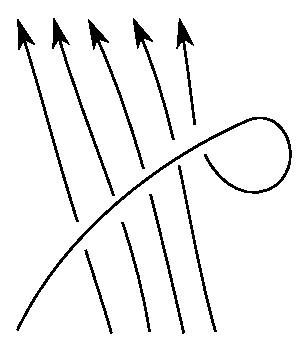
\includegraphics[width=0.2\linewidth]{torusbraid.eps}
    \caption{The diagram $\beta_5$}%
    \label{fig:torusbraid}
\end{figure}
Next, we will consider the diagram $\sigma_m$ below and denote its $n$-th power by $S_m^n$. These are required for the satellite construction for links, but we will not need it here.
\begin{figure}[H]
    \centering
    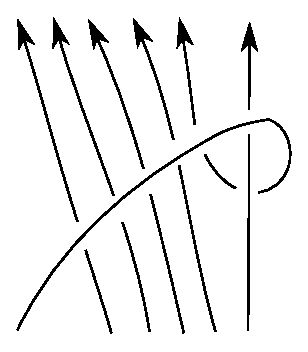
\includegraphics[width=0.2\linewidth]{splicebraid.eps}
    \caption{The diagram $\sigma_5$}%
    \label{fig:splicebraid}
\end{figure}

To conclude this section, we will explain how to actually construct the link diagram in the annulus for a non-reducible singularity. Let $C_1, \ldots, C_r$ be the branches of $C$ at $0$ and consider truncated Puiseux series
\[ y_i(x) = x^{\frac{q^i}{p^i}} (a_i + z_i(x^{\frac{1}{p^i}})). \]
Write $\alpha_i = \frac{q^i}{p^i}$ and consider the pairs $(\alpha_i, a_i)$. It is always possible to find a finite truncation of the Puiseux series that does not affect the topological type of the link, so the inductive process we will define is actually finite. For each $(\alpha, a)$, let $\qty{i_0, \ldots, i_n}$ be the set of indices with associated pair $(\alpha, a)$. Assume we have an annulus diagram $L_{(\alpha, a)}$ and set
\[ L_{\alpha} \coloneqq \prod_a L_{(\alpha, a)}. \]
We may assume that $\alpha_1 < \cdots < \alpha_k$, and the link $\mc{L}_C$ can be represented by the annulus diagram
\[ L_C \coloneqq S_{p^1}^{q^1} * (L_{\alpha_1}, S_{p^2}^{q^2} * (L_{\alpha_2}, \ldots, S_{p^{k-1}}{q^{k-1}} * T_{p^k}^{q^k} * L_{\alpha_k})). \]

\section{Some explicit calculations for the unknot and Hopf link}%
\label{sec:some_explicit_calculations_for_the_unknot_and_hopf_link}

The following is already apparently known.
\begin{prop}
    For any partition $\lambda$, 
    \[ \ev{Q_{\lambda}} = \prod_{\square \in \lambda} \frac{v^{-1} s^{c(\square)} - v s^{-c(\square)}}{s^{h(\square)} - s^{-h(\square)}}. \]
\end{prop}

Let $X \in \mc{C}_+$ be a counterclockwise-oriented diagram. Define the \textit{meridian operator} $\ms{M}_X$ on $\mc{C}_+$ by the construction below:
\begin{figure}[H]
    \centering
    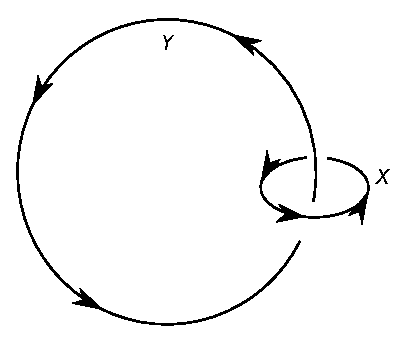
\includegraphics[width=0.2\linewidth]{mer6.eps}
    \caption{Meridian operator}%
    \label{fig:mer6}
\end{figure}
For a partition $\mu$, the Schur function $Q_{\mu}$ is an eigenvector for $\ms{M}_X$ with eigenvalue $t_{\mu}(X)$. Then the HOMFLY polynomial for the colored Hopf link decorated by $\mu, \lambda$ is simply $t_{\mu}(Q_{\lambda})(t_{\mu})$. In the remainder of this section, we will describe the operator $t_{\mu}$, which is a ring homomorphism $\mc{C}_+ \to \Lambda$. Define the function
\[ E_{\mu}(t) = \prod_{j=1}^{\ell(\mu)} \frac{1+v^{-1}s^{\mu_j - 2j + 1}t}{1+v^{-1}s^{-2j+1}t} \prod_{i \geq 0} \frac{1+v s^{2i+1}t}{1+v^{-1}s^{2i+1}t}. \]
Then we have $t_{\mu}(Q_{\lambda}) = s_{\lambda}(E_{\mu}(t))$, where for a power series $E(t) = \sum E_k t^k$, we write $s_{\lambda}$ as a polynomial in the $e_k$ and then substitute $e_k \gets E_k$.

\section{Behavior of links with respect to blowup}%
\label{sec:behavior_of_links_with_respect_to_blowup}

Having discussed the behavior of enumerative invariants with respect to blowups, we need to discuss the behavior of the link $\mc{L}_{C,0}$ with respect to blowing up the origin. Let $C_1, \ldots, C_r$ be the irreducible components of $C$ through $0$ and denote their strict transforms by $C_i'$. At each point $p_1, \ldots, p_e \in E$ (the exceptional divisor) let $D_k$ denote the singularity of $C' \cup E$ at $p_k$ and $B_k$ be the singularity of $C'$ at $p_k$. Choose (truncated) Puiseux expansions
\[ y_i(x) = x^{\frac{q^i}{p^i}} (a_i + z_i (x^{\frac{1}{p^i}})) \]
For each of the branches $C_i$. We may also assume that $\frac{q^i}{p^i} \geq 1$ for all $i$. If we blow up at the origin, consider the chart with coordinates $(x, y = xw)$. Substitution, we obtain the new Puiseux expansion
\[ w_i(x) = x^{\frac{q^i - p^i}{p^i}} (a_i + z_i(x^{\frac{1}{p^i}})) \]
for $C_i'$ at $p_k$. In particular, we obtain the relation
\[ [L_C] = \tau [L_{C'}] \qquad \tau(-) \coloneqq T_1^1 * (-). \]
If we perform deeper analysis, we obtain the following result:

\begin{prop}
    If any $\alpha_i = \frac{q_i}{p_i} > 1$, then we have
    \[ [L_C] = S_1^1 * (L_{B_1} \cdots L_{b_{e-1}}, \tau L_{B_e}). \]
    Otherwise, we have
    \[ [L_C] = S_1^1 * (L_{b_1} \cdots L_{B_e}, \emptyset) = T_1^1 * (L_{B_1} \cdots L_{B_e}). \]
\end{prop}

Now we will write down a blowup identity for links. The idea is to use the topological vertex (originally introduced by Aganagic-Klemm-Marino-Vafa) and its relationship with Chern-Sinons invariants of the unknot. For a partition $\mu$, define
\begin{align*}
    Z_{\mu}(q, Q) &= s_{\mu}(q^{\rho}) \prod_{\square \in \mu} (1 + Q q^{-c(\square)}) \\
    &= q^{\kappa_{\mu}/4} \prod_{\square \in \mu} \frac{1 + Q q^{-c(\square)}}{q^{h(\square)/2} - q^{-h(\square)/2}}.
\end{align*}
Here, $\kappa_{\mu} = 2 \sum_{\square \in \mu} c(\square)$. By the computation of the colored HOMFLY polynomial of the colored unknot (sorry), we obtain the identity
\begin{align*}
    Z_{\mu}(q=s^2, Q=-v^2) = v^{\abs{\mu}} \ev{Q_{\mu}}.
\end{align*}

\section{Relation between PT theory and HOMFLY}%
\label{sec:relation_between_pt_theory_and_homfly}

We will prove a relationship between the PT partition function for $C$-framed stable pairs in $Y = \mc{O}_{\P^1}(1) \oplus \mc{O}_{\P^1}(1)$ and the HOMFLY polynomial for $\mc{L}_{C,0}$. We will focus on the simplest case of a node with two branches. The general case reduces to this one by careful checking of what happens on both sides under blowup of $C$ at $0$.

\begin{prop}
    We have the identity (possibly up to monomials)
    \[ \ms{Z}'(Y, C; q, Q=0) = {(-1)}^{\ep} s^b \ev{[L_C * Q_{{(1)}^t}]}^{\mr{low}}, \]
    where the superscript low means we take the lowest degree terms.
\end{prop}

We only need to prove this for the unknot and the Hopf link.

\begin{proof}
    This apparently follows from the fact that the topological vertex calculates both the $v=0$ specialization of HOMFLY of the Hopf link and the stable pairs vertex. See the references to Maulik's paper for a reference.
\end{proof}

\chapter{Che (Oct 19): Braid varieties and Khovanov-Rozansky homology}%
\label{cha:che_oct_19_braid_varieties_and_khovanov_rozansky_homology}

\section{Khovanov-Rozansky homology}%
\label{sec:khovanov_rozansky_homology}

Let $G = GL_n$ and $\h$ be the Cartan. Write $R = \C[\h] = \C[x_1, \ldots, x_n]$, and this has an action of the Weyl group permuting the coordinates. We will specify $\deg x_i = 2$. We may now define Soergel bimodules
\[ B_i = R \otimes_{R^{s_i}} R(1). \]
Now define $T_i = [B_i(-1) \to R]$ by $1 \otimes 1 \mapsto 1$ and $T_i^{-1} = [R \to B_i(-1)]$ by $1 \mapsto x_i \otimes 1 - 1 \otimes x_{i+1}'$. We may now form the Rouquier complex for a braid $\beta = \sigma_{i_1} \cdots \sigma_{i_k}$ as
\[ T_{\beta} = T_{i_1} \otimes_R \cdots \otimes T_{i_k}. \]
For example, if $\beta = \sigma^2$, then we have
\[ T_{\beta} = [B(-1) \otimes B(-1) \to B(-1) \oplus B(-1) \to R] = [B(-3) \to B(-1) \to R]. \]
We may now take the Hochschild homology $\mr{HH}^i(T_{\beta})$. We will mostly be concerned with $\mr{HH}^0(M) = \Hom(R, M)$. Continuing our example, we have
\[ HH^0(T_{\beta}) = [R(-4) \xrightarrow{0} R(-2) \xrightarrow{x_1 - x_2} R]. \]
We are finally able to define the \textit{Khovanov-Rozansky homology}
\[ \mr{HHH}^*(\beta) \coloneqq H^*(\mr{HH}^*(\beta)). \]
This has gradings $A$ for the Hochschild grading, $Q$ for the internal degree in $R$, and $T$ for the homological grading. Continuing our example again, we have
\[ \mr{HHH}^{A=0}(\beta) = \frac{1}{1-Q^2} - \frac{Q^4 T^{-2}}{{(1-Q^2)}^2}. \]

\begin{rmk}
    We will usually multiply our $\mr{HHH}$ by $1-Q^2$ as a useful normalization. This is a consequence of us considering $G = GL_n$ instead of $G = SL_n$.
\end{rmk}

\section{Braid varieties}%
\label{sec:braid_varieties}

Write $B_i(z)$ for the matrix with $1$s on the diagonal except for a $\begin{psmallmatrix}
    0 & 1 \\ 1 & z
\end{psmallmatrix}$ block on the diagonal in the $i, i+1$ positions. Given $\beta = \sigma_{i_1} \cdots \sigma_{i_k}$, we consider the matrix
\[ B_{\beta}(z_1, \ldots, z_k) = B_{i_1}(z_1) \cdots B_{i_k}(z_k). \]
Then we may define the \textit{braid variety}
\[ X(\beta) \coloneqq \qty{(z_1, \ldots, z_k) \mid B_{\beta}(z_1, \ldots, z_k) \text{ is upper triangular}}. \]
For example, if $\beta = \sigma^2$ for $2$ strands, we have
\[ \mqty(0 & 1 \\ 1 & z_1) \mqty(0 & 1 \\ 1 & z_2) = \mqty(1 & z_2 \\ z_1 & 1 + z_1 z_2), \]
and so 
\[ X(\beta) = (z_1 = 0) \subseteq \C^2. \]
Similarly, for $\beta = \sigma^3$, we have the matrix
\[ \mqty(0 & 1 \\ 1 & z_1) \mqty(0 & 1 \\ 1 & z_2) \mqty(0 & 1 \\ 1 & z_3) = \mqty(z_2 & 1+z_2z_3 \\ 1 + z_1 z_2 & z_1 + z_3 + z_1 z_2 z_3), \]
and thus we have $X(\beta) = (1 + z_1 z_2 = 0) \times \C_{z_3}$. Similarly, we may compute
\[ X(\sigma^4) = \qty{z_1 + z_3 + z_1 z_2 z_3 = 0} \times \C_{z_4} = \qty{1 + z_2 z_2 \neq 0} \times \C_{z_4}. \]

These braid varieties come with a torus action. We would like to write
\[ \mqty(\dmat{t_1,\ddots,t_n}) B_i(z) = B_i(z') \mqty(\dmat{t_1',\ddots,t_n'}). \]
For example, we have
\[ \mqty(\dmat{t_1,t_2}) \mqty(0 & 1 \\ 1 & z) = \mqty(0 & t_1 \\ t_2 & t_2 z) = \mqty(0 & 1 \\ 1 & \frac{t_2}{t_1}z) \mqty(\dmat{t_2,t_1}). \]
Doing this on $B_{\beta}(z_1, \ldots, z_k)$, we obtain an action of $T = {(\C^{\times})}^n$ on $X(\beta)$. Continuing our example, we have
\[ z_1 \mapsto \frac{t_2}{t_1} z_1, \qquad z_2 \mapsto \frac{t_1}{t_2} z_2, \qquad z_3 \mapsto \frac{t_2}{t_1} z_3, \qquad\ldots \]
Here are some facts:
\begin{enumerate}
    \item Under mild assumptions, $X(\beta)$ is smooth.
    \item If $\beta$ closes to a knot, then the action of $T$ is free.
\end{enumerate}

We are now ready to state the main result.
\begin{thm}
    We have an equality
    \[ \operatorname{gr}_w H_T^*(X(\beta)) \cong \mr{HHH}^{A=n}(\beta) \]
    up to a global shift in grading, where $w$ is the weight filtration.
\end{thm}

\section{Mixed Hodge Structures}%
\label{sec:mixed_hodge_structures}

To understand the weight filtration, we will discuss mixed Hodge structures. For a smooth projective variety $X$ of dimension $n$, recall the \textit{Hodge decomposition}
\[ H^k(X, \C) = \bigoplus_{p+q=k} H^p(X, \Omega^q_X). \]
Of course, for general $X$ which are not necessarily smooth or projective, this decomposition will fail. In this case, there is a \textit{weight filtration}
\[ 0 = W_{-1} \subseteq W_0 \subseteq \cdots \subseteq W_{2k} = H^k(X, \C) \]
which morally measures how much the Hodge decomposition fails.

\begin{thm}
    Let $X$ be a smooth algebraic variety inside a smooth and projective $\ol{X}$ such that $D = \ol{X} \setminus X$ is a normal crossings divisor. Write $D = \bigcup_i D_i$ as a union of its irreducible components. Then there exists a spectral sequence
    \[ E_1^{-p,q} = H^{q-2p}(D^{(p)}) \Rightarrow \mr{gr}_w^q H^{q-p}(X) \]
    which collapses at the $E_2$ page. Here, $D^{(p)}$ is the locus of the $p$-fold intersection.
\end{thm}

Note that our spectral sequence looks like
\begin{equation*}
\begin{tikzcd}
    H^0(D^{(2)}) \ar{r} & \vdots \\
    0 & \vdots \\
    0 & H^0(D^{(1)}) \ar{r} & H^2(\ol{X}) \\
    0 & 0 & H^1(\ol{X}) \\
    0 & 0 & H^0(\ol{X})
\end{tikzcd} \implies
    \begin{tikzcd}
        \vdots & \vdots \\
        \vdots & \vdots \\
        \mr{gr}_w^2 H^1 & \mr{gr}_w^2 H^2 \\
        0 & \mr{gr}_w^1 H^1 \\
        0 & \mr{gr}_w^0 H^0.
    \end{tikzcd}
\end{equation*}

For example, when $X = \C^{\times}$ and $\ol{X} = \P^1$, we have $D = 0 + \infty$, and so we obtain
\begin{equation*}
\begin{tikzcd}
    2 \ar{r} & 1 \\
    0 \ar{r} & 0 \\
    0 \ar{r} & 1 
\end{tikzcd} \implies
\begin{tikzcd}
    1 & 0 \\
    0 & 0 \\
    0 & 1 
\end{tikzcd}
\end{equation*}
and for example, $\mr{gr}_w^2 H^1(\C^{\times}) = \C$.

\section{Sketch of proof of main theorem}%
\label{sec:sketch_of_proof_of_main_theorem}

What we will do is to construct a Bott-Semelson variety $\mr{BS}(\beta)$ from the Khovanov-Rozansky homology, then as a fiber over the flag variety we will consider the brick variety of $\beta$, which is a compactification of $X(\beta)$.

\begin{defn}
    Given $\beta = \sigma_{i_1} \cdots \sigma_{i_k}$, define the \textit{Bott-Samelson variety}
    \[ \mr{BS}(\beta) = \qty{(F_0, \ldots, F_k) \mid F_i \in G/B, F_0 = F^{\mr{st}}, F_j \neq F_{j+1} \text{ only in the $i_j$th position}}. \]
\end{defn}

For example, when $\beta = \sigma_1 \sigma_2$, we have
\[ 
F_0 = (e_1) \subset (e_1, e_2) \subset (e_1, e_2, e_3)
F_1 = (e_2) \subset (e_1, e_2) \subset (e_1, e_2, e_3)
F_2 = (e_2) \subset (e_2, e_3) \subset (e_1, e_2, e_3).
\]
Then $(F_0, F_1, F_2) \in \mr{BS}(\beta)$. Now we define the open Bott-Samelson variety 
\[ \mr{OBS}(\beta) = \qty{(F_0, \ldots, F_k) \in \mr{BS}(\beta) \mid F_j \neq F_{j+1}}. \]
We have the projection $\mr{pr} \colon \mr{BS}(\beta) \to G/B$ sending a tuple of flags to $F_k$. Then we define
\[ \mr{brick}(\beta) = \mr{pr}^{-1} \delta(\beta) F^{\mr{st}}, \]
where $\delta(\beta) \in W$ is the Demazure product. Finally, define $\mr{brick}^0(\beta) = \mr{brick}(\beta) \cap \mr{OBS}(\beta)$.

\begin{thm}\leavevmode
    \begin{enumerate}
        \item $X(\ateb; \delta(\beta)) \cong \mr{brick}^0(\beta)$, where $\ateb$ is $\beta$ with the transpositions reversed.
        \item The complement $\mr{brick}(\beta) \setminus \mr{brick}^0(\beta)$ is a normal crossings divisor.
        \item The brick variety $\mr{brick}(\beta)$ has a stratification by $\mr{brick}(\beta')$ for subwords $\beta'$ of $\beta$ such that $\delta(\beta) = \delta(\beta')$.
    \end{enumerate}
\end{thm}

\begin{rmk}
    We define $X(\beta, w)$ for some $w \in W$ as
    \[ \qty{(z_1, \ldots, z_k) \mid B_{\beta}(z_1, \ldots, z_k) w \text{ is upper triangular}}. \]
    For example, we have $X(\sigma^3, (12)) = \qty{1 + z_1 z_2 \neq 0}$. On the other hand, $\mr{brick}(\sigma^3) = \P^1 \times \P^1$, $\mr{brick}(\sigma^2) = \P^1$, and $\mr{brick}(\sigma) = \mr{pt}$.
\end{rmk}

\begin{thm}
    As an $R-R$ bimodule, we have
    \[ H_T^*(\mr{BS}(\sigma_{i_1} \cdots \sigma_{i_k})) \cong R \otimes_{R^{s_{i_1}}} \cdots \otimes_{R^{s_{i_n}}} R. \]
\end{thm}

\chapter{Sam (Oct 26 and Nov 09): Finite dimensional type A rational Cherednik representations}

Let $R$ be the $A_{n-1}$ root system, $W$ be the Weyl group $S_{n-1}$, and $\h$ be the $n-1$-dimensional representation. Sitting inside $W$ there is a canonical set of generators.

\begin{defn}
    Given a constant $c$, define the \textit{rational Cherednik algebra} to be the algebra generated by $\mr{Sym}(\h^{*}) = \C[\h]$, $\mr{Sym}(\h) = \C[\h^{*}]$, and $\C W$ with the relations
    \begin{itemize}
        \item $[x_{i}, x_{j}] = 0 = [y_{i}, y_{j}]$;
        \item $w x w^{{-1}} = w(x)$ and $-w y w^{-1} = w(y)$;
        \item $[y,x] = \ev{y,x} - c \sum_{s \in S} \ev{y, \alpha_s} \ev{\alpha_s^{\vee}, x} s$,
    \end{itemize}
    where $x_1, \ldots, x_{n-1} \in \mr{Sym}(\h^*)$ and $y_1, \ldots, y_{n-1} \in \mr{Sym}(\h)$ are the canonical set of generators.
\end{defn}

This has some induced representations. If $\tau$ is a representation of $W$, then there is an action of $\C[\h^*] \rtimes W$ on $\wh{\tau}$, which is the same vector space. This is given by $P \mapsto P(0)$. Then we may define
\[ M(\tau) = H_c \otimes_{\C[\h^*] \rtimes W} \wh{\tau}. \]
Here are some basic properties:
\begin{enumerate}
    \item There is a grading where $x_i$ have degree $1$, $y_i$ have degree $-1$, and $w$ has degree $0$.
    \item There is a filtration given by taking the total degree in $x$ and $y$.
\end{enumerate}

A stranger property is that there is some $\mf{sl}_2$-triple. Here, if 
\[ \mathbf{h} = \frac{1}{2} \sum_{i=1}^{n-1} x_i y_i + y_i x_i, \qquad E = -\frac{1}{2} \sum x_i^2, \qquad F = \frac{1}{2} \sum y_i^2, \]
then $E,\mathbf{h}, F$ is an $\mf{sl}_2$-triple. This integrates to an $SL(2, \C)$ action given by $x_i \mapsto y_i, y_i \mapsto -x_i$, which is called the \textit{Fourier transform}. 

\section{Relation to KZ-connection}%
\label{sec:relation_to_kz_connection}

Let $\C[\h] = H^0(\h) = M(\mr{triv})$ and define operators
\[ D_i \coloneqq \pdv{x_i} + c \sum_{j \neq i} \frac{s_{ij} - \mr{Id}}{x_i - x_j}. \]
These are called the \textit{Dunkel operators}.

\begin{exer}
    If $y_i = D_i$, then this gives the relations in the rational DAHA for $\mf{gl}_{n-1}$.
\end{exer}

\begin{cor}
    Because $[D_i, D_j] = 0$, then a module $M(\tau)$ gives us a bundle with meromorphic connection on $\h$. Note that the poles along hyperplanes are of order $1$, which means we have regular singularities and thus we can study representations of DAHA using the Riemann-Hilbert correspondence.
\end{cor}

\section{Background on $\mc{H}_{q_c}$-representations}%
\label{sec:background_on_h__q_c_representations}

The Hecke algebra $\mc{H}_q$ is a deformation of $S_n = \mc{H}_1$. Given a parameter $c$, we obtain a parameter $q_c = e^{2\pi i c}$. Now there is a theory of Specht-modules.

\begin{thm}[Dipper-James]\leavevmode
    \begin{enumerate}
        \item There is a flat (over $\A^1_q$) family $S^{\lambda}$ of $\mc{H}_Q$-modules nduced by any partition $\lambda$ of $n$. This exhausts without repetition the representations for $q$ not a root of unity and agrees with the usual Specht module $S^{\lambda}$ for $q = 1$.
        \item When $q$ is a root of unity, these are not always irreducible. If $e$ is the order of $q$ and $\lambda$ is $e$-regular (the multiplicity of every $\lambda^{(i)}$ is less than $e$), then $S^{\lambda}$ is irreducible.
        \item There always exists a simple quotient $D^{\lambda}$ of $S^{\lambda}$.
        \item There is a bijection between blocks of representations of $\mc{H}_q$ and $e$-cores. An $e$-core is a partition $\lambda$ of $n$ without $e$-hooks.
    \end{enumerate}
\end{thm}

For $e = n$, either $\lambda$ is an $e$-core or $\lambda$ is one of $(n), (n-1,1), \ldots, (1,\ldots,1)$. In this case, we obtain the representations $\bigwedge^0 \h, \bigwedge^1 \h, \ldots, \bigwedge^{n-1} \h$. Clearly $\bigwedge^0 \h$ is the trivial representation, $\bigwedge^1 \h = \h$, ad $\bigwedge^{n-1} \h$ is the sign representation.

\begin{prop}
    The composition series of $S^{\lambda^i}$ is given by
    \[ 0 \to D^{\lambda^{i-1}} \to S^{\lambda^i} \to D^{\lambda^i} \to 0 \]
    whenever these are defined. Moreover, $D^{\lambda^{-a}} = 0, D^{\lambda^{n-1}} = 0$, but the other $D^{\lambda^i} \neq 0$ for $i < n-1$.
\end{prop}

\begin{exm}
    For $n = 3$, we have the composition series
    \[ 0 \to D^{(3)} \to S^{(2,1)} \to D^{(2,1)} \to 0. \]
    If we take $\mc{H}_{\zeta_3}$, the action on $\h$ has a trivial $1$-dimensional submodule.
\end{exm}

\section{The KZ functor}%
\label{sec:the_kz_functor}

Consider the weight zero summand $\mc{O}(\mc{H}_c)$ of category $\mc{O}$. Then the monodromy gives us a local system on $\h^{\mr{reg}} = \h \setminus \bigcup H_{\alpha}$. Remember that the root hyperplanes were the singularities of our connection $D_i$. Given $M(\tau)$, we obtain the module
\[ \C[\h^{\mr{reg}}] \otimes_{\C[\h]} M(\tau), \]
and in fact this is the monodromy. This gives us a $W$-equivariant local system on $\h^{\mr{reg}}$, and these are the same thing as $\ms{Rep}(\pi_1(\h^{\mr{reg}} / W)) = \ms{Rep}(B_n)$. We claim that this gives an equivalence
\[ \mc{O}(H_c) / \mr{tors} \xrightarrow{\sim} \ms{Rep}(\mc{H}_{q_c}). \]

\begin{proof}
    We will give a ``proof'' of this result. The first thing we need to prove that $(T_i - q_c)(T_i - 1)$, where $T_i$ is the monodromy around $\gamma_i$, where $\gamma_i$ is a small loop around $H_{\alpha_i}$. In the $n=2$ case, our Dunkel operator is simply
    \[ D = \pdv{x_i} + c \frac{s - \mr{Id}}{\alpha}. \]
    For the trivial and nontrivial representation of $\Z/2\Z$, we obtain either
    \[ D = \begin{cases}
        \pdv{x_i} + \frac{2c}{\alpha} \\
        \pdv{x_i}.
    \end{cases}
    \]
    But now we may compute the monodromy. In the case of $\pdv{x_i}$, we have trivial monodromy. In the harder case, if we complexify to $z$ and take $\xi = \sqrt{z}$ (corresponding to going halfway around a hyperplane), then we have
    \[ D = \pdv{z} + \frac{2c}{z} \mapsto \pdv{\xi} + \frac{c}{\xi}. \]
    This clearly has monodromy $e^{2\pi i c} = q_c$ because we have the fundamental solution $\phi = e^{c \log \xi}$. Then there is something that reduces the general case to this calculation.

    This functor factors through torsion because torsion is the kernel of $\C[\h^{\mr{reg}}] \otimes -$. This was the first step, so this is clear. We now prove equivalence. This follows from the Riemann-Hilbert correspondence once we prove regularity at infinity in some compactification. This computation is omitted.
\end{proof}

We will use
\[ 0 \to D^{\lambda^{i-1}} \to S^{\lambda^i} \to D^{\lambda^i} \to 0 \]
to give a representation of $L(\mr{triv}) = M(\mr{triv}) / J(\mr{triv})$.

\begin{thm}[BGG (BEG)]
    There is a resolution
    \[ M(\Lambda^{n-1} \h) \to \cdots \to M(\Lambda^1 \h) \to M(\mr{triv}) \to L(\mr{triv}). \]
\end{thm}

This result follows from the fact that the block of representations of the Hecke algebra has $n-2$ simple representations, so once we finish at $M(\mr{triv})$, we must have a torsion module, which must be $L(\mr{triv})$. If $c = \frac{m}{n} > 0$ and $(m,n) = 1$, then $L(\mr{triv})$ is finite-dimensional.

\begin{exm}
    By definition, it is clear that $M(\mr{triv}) = \C[\h]$. Thus the BGG resolution is the Koszul resolution of $\Spec L(\mr{triv})$. When $n = 2$ and $c = \frac{2}{3}$, the image $\Im(M(\Lambda^1 \h)\to M(\mr{triv}))$ is the ideal 
    \[ (u_1^2 - u_2^2, u_1^2 - u_1 u_2) \subseteq \C[\h], \]
    where $u_1, u_2$ are $x_1 - x_2, x_2 - x_3$. These are just two reducible pairs of lines, and so then if we take $\Spec L_{2/3}(\mr{triv})$, we obtain the subscheme defined by the above ideal. Clearly $L_{2/3}(\mr{triv})$ is the ring of functions on this scheme.
\end{exm}

In the $A_3$ case, we have $\Spec L_{r/4}(\mr{triv})$ is a local complete intersection. This is derived smooth, and so we have some kind of Poincar\'e duality.

\section{Characters for $H_c$ representations}%
\label{sec:characters_for_h_c_representations}

Let $\mathbf{h} = \frac{1}{2} \sum x_i y_i$, where $y_i$ is a basis for $\h^*$ and $x_i$ is the dual basis. Then $V \in \mc{O}(H_c)$ splits as
\[ V = \bigoplus_a V_a, \]
where $\mathbf{h}$ acts by $a$. Because $W$ commutes with $\mathbf{h}$ we can keep track of the $\mathbb{h}$-grading and $W$-characters.

\begin{defn}
    We define 
    \[ \mr{Tr}_V (w \circ q^{\mathbf{h}}) \coloneqq \sum_a q^a \mr{Tr}^W(w, V_a). \]
\end{defn}


Now we will define the character for $M_c(\tau)$. We an $\mathbf{h} \times W$-module, we have
\[ M_c(\tau) \cong \C[\h] \otimes \tau. \]
Therefore we have
\[ \mr{Tr}_{M_c(\tau)}(w \cdot q^{\mathbf{h}}) = \frac{\kappa(c, \tau) \mr{Tr}^W(w, \tau)}{\det_{\h} (1-wq)}. \]
Here, $\kappa(c, \tau)$ is the lowest weight.

We will now compute $\kappa$ for $\tau = \Lambda^{\bullet} \h$. To begin, suppose that $\tau$ is the trivial representation. Then the lowest weight vector is $1$ and the $y_i$ act by $0$. We now have
\begin{align*}
    \mathbf{h} &= \frac{1}{2} \sum_{i=1}^{n-1} x_i y_i + y_i x_i \\
    &= \frac{1}{2} \sum_{i=1}^{n-1} [y_i, x_i] \\
    &= \frac{1}{2} \sum_{i=1}^{n-1} \qty( \ev{y_i, x_i} - c \sum_{s \in S} \ev{y_i, \alpha_s^{\vee}} \ev{\alpha_s, x_i} s) \\
    &= \frac{1}{2} \qty(n-1-c \cdot 2 \frac{n(n-1)}{2}).
\end{align*}
Next, we use the Koszul-BGG resolution and see that
\[ \kappa(c, \Lambda^i \h) = \kappa(c, \mr{triv}) + c \cdot n \cdot i = \frac{n-1}{2} + cn\qty(i - \frac{n-1}{2}). \]

Finally, we compute the characters for $L_c(\mr{triv})$ and prove that they exhaust finite-dimensional representations. Suppose $[L] \in \mc{O}(H_c)$ is finite-dimensional. For $c > 0$ we have $H_c \simeq H_{-c}$. We know that $L$ is in the block containing $M_c(\Lambda^i \h)$. Therefore we have
\[ [L] = \sum_{i=1}^{n-1} a_i [M_c(\Lambda^i \h)]. \]
This gives us
\begin{align*}
    \mr{Tr}_L(1 \cdot q^{\mathbf{h}}) = \frac{1}{\det_{\h}(1-q)} \sum_{i=1}^{n-1} a_i q^{\kappa(c, \mr{triv}) + cni} \binom{n-1}{i}.
\end{align*}
This is a degree $n-1$ polynomial $Q(q^{cn})$ and also that the trace is finite as $q \to 1$, so in fact $Q(q^{cn}) \propto (1-q)^{n-1}$. Therefore $a_i = {(-1)}^i$ assuming that $\dim L > 0$ and $L$ is simple. But now we see that $L = L(\mr{triv})$, and so
\begin{align*}
    \mr{Tr}_{L_c(\mr{triv})} (w \cdot q^{\mathbb{h}}) = q^{\frac{n-1}{2} - \frac{cn(n-1)}{2}} \frac{\det_{\h} (1-wq^r)}{\det_{\h}(1-wq)}.
\end{align*}

\chapter{Cailan (Nov 09 and Nov 16): Torus knots and the rational DAHA}%
\label{cha:cailan_nov_09_torus_knots_and_the_rational_daha}

\section{Representation theory}%
\label{sec:representation_theory}

We will begin by changing Sam's formula until it is in the form that Cailan wants:
\begin{align*}
    \mr{Tr}_{L_{m/n}} (w \cdot q^{\mathbb{h}}) = q^{\frac{n-1}{2}(m-1)} \frac{\det_{\h} (1-wq^m)}{\det_{\h}(1-wq)}.
\end{align*}

\begin{defn}
    Let $L$ be a representation of $S_n$. Define $\mr{ch} \colon \ms{Rep}(S_n) \to \Lambda_n$ by
    \[ \mr{ch}(L) = \frac{1}{n!} \sum_{\theta \in S_n} \mr{Tr}_L(\theta) p_1^{k_1(\theta)} \cdots p_r^{k_r(\theta)}, \]
    where $p_i$ are the power sums and $k_i(\theta)$ is the number of cycles of length $i$ in $\theta$.
\end{defn}

\begin{rmk}
    We have $\mr{ch}(S^{\lambda}) = s_{\lambda}$. Also, $[S^{\lambda}]$ is a basis for $K_0(\ms{Rep}(S_n))$, and in fact, there is an isomorphism of Hopf algebras
    \[ \mr{ch} \colon K_0\qty( \bigoplus_{n \geq 0}\ms{Rep}(S_n)) \simeq \Lambda \]
    with the ring of symmetric polynomials in infinitely many variables.
\end{rmk}

\begin{lem}
    The reflection (representation) of $S_n$ is isomorphic to $\C^n / \C \cdot (x_1 + \cdots x_n)$.
\end{lem}

\begin{lem}
    Let $T \colon V \to V$ be a linear operator and let $V = V_1 \oplus \cdots \oplus V_k$ be a sum of $T$-invaraint subspaces. Then $\chi_T(q) = \chi_{T|_{V_1}}(q) \cdots \chi_{T|_{V_k}}(q)$.
\end{lem}

\begin{proof}
    Clearly $T - qI$ is a block matrix.
\end{proof}

\begin{prop}
    For each $\sigma \in S_n$ acting in the reflection representation $h$, we have
    \[ \det(1-q \sigma) = \frac{1}{1-q} \prod_i (1-q^i)^{k_i(\sigma)}. \]
\end{prop}

\begin{prop}
    For $A \colon V \to V$ with $\dim V = n$, we have
    \[ \det(I - qA) = (-q)^n \chi_A(q^{-1}). \]
\end{prop}

\begin{proof}
    Note that $\C^n = h \oplus \mr{triv}$. Therefore by the previous lemma, we have
    \[ \det_h(1-q \sigma) = \frac{\det_{\C^n} (1-q\theta)}{\det_{\mr{triv}}(1-q \theta)} = \frac{\det_{\C^n}(1-q\theta)}{1-q}. \]
    By conjugation invariance of the characteristic polynomial, it is invariant under permutation matrices, which corresponds to conjugation in $S_n$, and so the trace depends only on the cycle type. For each cycle $c$ in $\sigma$ of length $i$, there exists a $\sigma$-invariant subspace $V_c$ of $\C^n$ of dimension $i$. Clearly the trace only depends on the length $i$. Also, we know that
    \[ \C^n = V_{c_1} \oplus \cdots \oplus V_{c_m} \]
    and each $V_{c_i}$ is $\sigma$-invariant. Using the lemma again, we have
    \[ \det_{\C^n} (1-q \sigma) = \prod_i \det_{\C^i} (I - q (1 2 \cdots i))^{k+i(\theta)}. \]
    It is easy to check that $\chi_{T_i}(q) = {(-1)}^i (q^i - 1)$, and therefore we have
    \[ \det_{\C^i}(1-q (1 2 \cdots i)) = (-1)^i \chi_{T_i}(q) = q^i \qty(\frac{1}{q^i} - 1) = 1-q^i, \]
    as desired.
\end{proof}

\begin{thm}
    Let $F_{m/n}(q, p_i) = \mr{gch}(L_{m.n})$ be the graded Frobenius character. This is equal to $\sum_i \mr{ch}((L_{m/n})_i) q^i$. Fixing $m$, we claim that the function
    \[ F_m(q, p_i) \coloneqq \sum_{n=0}^{\infty} F_{m/n}(q, p_i) z^n \]
    satisfies the identity
    \[ F_m(q, p_i) = \frac{1}{[m]_q} \prod_{j=0}^{m-1} \prod_{k=1}^{\infty} \frac{1}{1- q^{j+\frac{1-m}{2}} z x_k}, \]
    where $[m]_q = \frac{q^{m/2} - q^{-m/2}}{q^{1/2} - q^{-1/2}}$.
\end{thm}

\begin{proof}
    Let $\delta_{m, n} = \frac{(m-1)(n-1)}{2}$. Using Sam's formula, we have
    \begin{align*}
        \sum_i \mr{Tr}(\sigma, (L_{m/n})_i) q^i &= q^{-\delta_{m.n}} \frac{\det_h (1-q^m \sigma)}{\det_h (1-q \sigma)} \\
        &= q^{-\delta_{m,n}} \frac{1-q}{1-q^m} \prod_i \qty(\frac{1-q^{m_i}}{1-q^i})^{k_i(\sigma)}.
    \end{align*}
    Therefore 
    \begin{align*}
        F_{m/n}(q, p_i) &= \sum_i \frac{1}{n!} \sum_{\sigma \in S_n} \mr{Tr}(\theta, (L_{m/n})_i) p_1^{k_1(\sigma)} \cdots p_r^{k_r(\sigma)} q^i \\
        &= \frac{1}{n!} \sum_{\theta \in S_n} \frac{q^{\frac{n(1-m)}{2}}}{[m]_q} \prod_i \qty(\frac{1-q^{m_i}}{1-q^i} p_i)^{k_i(\sigma)}.
    \end{align*}
    By an easy exercise, it is easy to see that $q^{-\delta_{m,n}} \frac{1-q}{1-q^m} = \frac{q^{\frac{n(1-m)}{2}}}{[m]_1}$. Therefore we have
    \begin{align*}
        F_m(q, p_i) &= \sum_{n=0}^{\infty} \frac{1}{n!} \sum_{\sigma \in S_n} \frac{q^{\frac{n(1-m)}{2}}}{[m]_q} \prod_i \qty(\frac{1-q^{m_i}}{1-q^i} p_i)^{k_i(\theta)} z^n \\
        &= \sum_{n = 0}^{\infty} \frac{1}{n!} \sum_{\lambda \vdash n} \frac{n!}{\prod_i i^{k_i(\lambda)} k_i(\lambda)!} \frac{q^{\frac{n(1-m)}{2}}}{[m]_q} \prod_i \qty(\frac{1-q^{m_i}}{1-q^i} p_i)^{k_i(\lambda)} z^n \\
        &= \frac{1}{[m]_q} \sum_{n=0}^{\infty} \sum_{\lambda \vdash n} \prod_i \frac{1}{k_i(\lambda)!} \qty(\frac{(1-q^{m_i}) p_i q^{\frac{i(1-m)}{2}} z^i}{(1-q^i) i})^{k_i(\lambda)}.
    \end{align*}
    Using the fact that $\sum_i i k_i(\lambda) = n$, we have
    \begin{align*}
        \prod_i \frac{1}{1-z^i} = \sum_{n=0}^{\infty} \qty(\sum_{\lambda \vdash n} i) z^n = \sum_{n=0}^{\infty} \sum_{\lambda \vdash n} \prod_i (z^i)^{k_i(\lambda)}.
    \end{align*}
    This tells us that
    \[ \prod_i \frac{1}{1-f(q, i) z^i} = \sum_{n=0}^{\infty} \sum_{\lambda \vdash n} \prod_i (f(q, i) z^i)^{k_i(\lambda)}. \]
    We now have
    \begin{align*}
        F_m(q, p_i) &= \frac{1}{[m]_q} \exp \qty(\sum_{i=1}^{\infty} \frac{(1-q^{m_i})p_i q^{\frac{i(1-m)}{2}} z^i}{(1-q^i) i}) \\
        &= \frac{1}{[m]_q} \prod_{j=0}^{m-1} \exp \qty(\sum_{i=1}^{\infty} \frac{q^{ij} p_i q^{\frac{i(1-m)}{2}} z^i}{i}) \\
        &= \frac{1}{[m]_q} \prod_{j=0}^{m-1} \exp\qty(\sum_{i=1}^{\infty} \frac{(q^{j + \frac{1-m}{2}} z)^i}{i} p_i) \\
        &= \frac{1}{[m]_q} \prod_{j=0}^{m-1} \prod_{k=1}^{\infty} \exp \log \qty(\frac{1}{1-q^{j + \frac{1-m}{2}} z x_k}). \qedhere
    \end{align*}
\end{proof}

\begin{rmk}
    The Frobenius character is really the same information as $\qty{\chi_L(g)}_{g \in S_n}$. For $\mr{id} = (1^n)$, we see that $\ev{p_1^n} \on{ch} L = \frac{\dim L}{n!}$, and thus $\dim L = n! \ev{\on{ch} L, p_1^n}$. Also, $\on{\ch}(L)$ is the generating function for
    \begin{equation*}
    \begin{tikzcd}
        K_0\qty(\bigoplus_{n \geq 0} \on{Rep} S_n) \ar{dr}{\on{ch}} & & K_0(\ms{Rep}^{\mr{poly}}(GL(m))) \ar{dl}{\Tr(\mr{diag}(x_1, \ldots, x_n), -)} \\
        & \mr{Sym}.
    \end{tikzcd}
    \end{equation*}
\end{rmk}

\begin{thm}
    As a graded $S_n$-representation, we have
    \[ L_{m/n} = \frac{1}{[m]_q} \bigoplus_{\lambda \vdash n} s_{\lambda}(q^{\frac{1-m}{2}}, q^{\frac{3-m}{2}}, \cdots, q^{\frac{m-1}{2}}) S^{\lambda}. \]
\end{thm}

\begin{proof}
    It suffices to prove this at the level of the Frobenius character. We have the Cauchy identity
    \[ \prod_{k, j} \frac{1}{1-x_k y_j} = \sum_{\lambda} s_{\lambda}(x_1, \ldots), s_{\lambda}(y_1, \ldots), \]
    and here we will specialize to
    \[ y_j = \begin{cases}
        z q^{j + \frac{1-m}{2}} & 0 \leq j < m \\
        0 & j \geq m.
    \end{cases}
    \]
    This implies that
    \begin{align*}
        \mr{gch}(L_{m/n}) &= \ev{z^n} F_m(q, p_i) \\
        &= \ev{z^n} \frac{1}{[m]_q} \prod_{j=0}^{m-1} \prod_{k=1}^{\infty} \frac{1}{1-q^{j+\frac{1-m}{2}} z x_k} \\
        &= \ev{z^n} \frac{1}{[m]_q} \sum_{\lambda} s_{\lambda}(x_1, \ldots) s_{\lambda}(zq^{\frac{1-m}{2}}, \ldots, zq^{\frac{m-1}{2}}) \\
        &= \ev{z^n} \frac{1}{[m]_q} \sum_n \sum_{\lambda \vdash n} z^n s_{\lambda}(q^{\frac{1-m}{2}}, \ldots, q^{\frac{m-1}{2}}) s_{\lambda}(x_1, \ldots) \qedhere
    \end{align*}
\end{proof}

\begin{prop}
    We have 
    \[ s_{\lambda}(q^{\frac{1-m}{2}}, \ldots, q^{\frac{1-m}{2}}) = \prod_{(i,j) \in \lambda} \frac{[m+i-j]_q}{[h_{\lambda}(i, j)]_q}. \]
\end{prop}

\begin{exm}
    We have $L_{3/2} = (q+q^{-1}) S^{(2)} \oplus S^{(1,1)}$.
\end{exm}

\section{HOMFLY polynomial of torus knots}%
\label{sec:homfly_polynomial_of_torus_knots}

\begin{defn}
    We will define the HOMFLY polynomial using the same skein relations as before but with $P(\mr{unknot}) = 1$.
\end{defn}

\begin{exm}
    For the trefoil $T(2,3)$ we have $P(T(2,3)) = a^2(q^2 - q^{-2} - a^2)$.
\end{exm}

\begin{defn}
    Define $H_q(n)$ to be the quotient of $\Z[q^{\pm}][B_n]$ by the relation $\sigma_i^2 = (q-1) \sigma_i + q$. Let $g_i = [\sigma_i] \in H_q(n)$.
\end{defn}

Here, $q$ will always be generic, unlike in Sam's lecture.

\begin{defn}
    The \textit{Jones-Ocneanu trace} $\tr \colon \bigcup_{n \geq 1} H_q(n) \to \Z[q^{\pm}][z]$ is the unique linear map such that $\tr(ab) = \tr(ba)$, $\tr(1) = 1$, and $\tr(x g_n) = z \tr(x)$ for any $x \in H_q(n)$.
\end{defn}

\begin{thm}[Jones]
    Let $B \in B_n$. Let $\chi_B(q, \lambda) = f(q, \lambda) \tr([B])|_{z = \frac{1-q}{1-\lambda q}}$. Then
    \[ P(\wh{B})(a,q) = \chi_B\qty(q^2, \frac{a^2}{q}). \]
\end{thm}

\begin{thm}[Ocneanu]
    Let $x \in H_q(n)$. Then
    \[ \tr(x) = \sum_{\lambda \vdash n} \Tr_{S^{\lambda}(q)} \prod_{(i,j) \in \lambda} \frac{q^i(1-q+z) - q^j z}{1-q^{{h_{\lambda}(i,j)}}}. \]
\end{thm}

\begin{proof}
    We know that $H_q(n) = \bigoplus_{\lambda \vdash n} \End(S^{\lambda}(q))$ for $q$ generic and any $f \colon M_k(\C) \to \C$ satisfying commutativity is a scalar multiple of the trace.
\end{proof}

\begin{defn}
    We define $T(m, n)$ to be the closure of the braid $(\sigma_1 \cdots \sigma_{n-1})^m$. 
\end{defn}

\begin{rmk}
    $T(m,n)$ is a knot if and only if $(m,n) = 1$. In addition, $T(m,n) = T(n,m)$.
\end{rmk}

Let $\pi_{\lambda} \colon H_q(n) \to \End(S^{\lambda}(q))$.
\begin{lem}
    Fix $\lambda \vdash n$. Define $e_i = \frac{1 + \pi_{\lambda}(g_i)}{1+q}$. Then $e_i^2 = e_i$. Moreover, let $\dim S^{\lambda}(q) = d$ and $\on{rk}_{S^{\lambda}(q)} e_i = r$. Then
    \[ \pi_{\lambda}((g_1 \cdots g_{n-1})^n) = q^{\frac{rn(n-1)}{d}} \mr{id}_{S^{\lambda}(q)}. \]
\end{lem}

\begin{proof}
    We omit checking that $e_i$ is idempotent. Next, we have a very important fact that $FT_n = (\sigma_1 \cdots \sigma_{n-1})^n$ is central in $B_n$. Therefore, $\pi_{\lambda}((g_1 \cdots g_{n-1})^n) = c \mr{id}_{S^{\lambda}}$ for some $c \in C$. By definition, $\pi_{\lambda}(g_i) = q e_i - (1-e_i)$, and so in some basis of $S^{\lambda}(q)$, we have
    \[ \pi_{\lambda}(g_i) = \mqty(\dmat{q,\ddots,q,-1,\ddots,-1}). \]
    This implies that $\det \pi_{\lambda}(g_i) = \pm q^r$, and therefore $\det(\pi_{\lambda}((g_1 \cdots g_{n-1})^n)) = q^{rn(n-1)}$, so $c^d = q^{rn(n-1)}$, and thus $c = w(q) q^{rn(n-1)/d}$, where $w \colon \C \to \zeta_d$ is continuous. But now $w$ is constant because $\C$ is connected and $\zeta_d$ is discrete.

    We can now thus evaluate at $q = 1$. Note that $g_1 \cdots g_{n-1} = (1 n (n-1) \cdots 2)$ at $q = 1$, and therefore because $(1 n \cdots 2)^n = 1$, we see that $c = 1$.
\end{proof}

\begin{lem}
    The matrix $A_{\lambda}(q) = q^{-r(n-1)/d} \pi_{\lambda}(g_1 \cdots g_{n-1})$ is conjugate to the matrix for $(1 n \cdots 2)$ acting on $S^{\lambda}$.
\end{lem}

\begin{proof}
    We know that $A_{\lambda}(q)^n - I = 0$, and thus $A_{\lambda}(q)$ is diagonalizable. In particular, the conjugacy class is determined by the eigenvalues and their multiplicities. By the same continuity argument, we can evaluate at $q = 1$.
\end{proof}

\begin{cor}
    Suppose $(m,n) = 1$. Then 
    \[ \Tr(\pi_{\lambda}((g_1 \cdots g_{n-1})^m)) = \begin{cases}
        (-1)^a a^{m r(n-1)/d} & \lambda = H_{a,b} \\
        0 & \text{otherwise}.
    \end{cases} \]
\end{cor}

\begin{proof}
    By the lemma, we have
    \begin{align*}
        \mr{Tr}(\pi_{\lambda}((g_1 \cdots g_{n-1})^m)) &= q^{mr(n-1)/d} \Tr_{S^{\lambda}}((n n-1 \cdots 1))^m \\
        &= q^{mr(-1)/d} \sum_i \lambda_i^m \\
        &= \sum \lambda_i
    \end{align*}
    by Galois theory, where $\lambda_i$ are the eigenvalues of $(n \cdots 1)$. Now everything follows from the Murnaghan-Nakayama rule.
\end{proof}

\begin{thm}
    Suppose $(m,n) = 1$. Then 
    \begin{align*} 
        P(T_{m,n})(a,q) &= \frac{a^{m(n-1)} \ev{1}_q}{\ev{n}_q} \sum_{b=0}^{n-1} (-1)^{n-1-b} \frac{q^{-m}(2b-n+1)}{\ev{b}_q \ev{n-1-b}_q} \prod_{j=b-n-1,j \neq 0} (q^j a - q^{-j} a^{-1}) \\
        &= \frac{1 + \pi_{\lambda}(g_i)}{1+q}.
    \end{align*}
    Here, $\ev{n} = q^n - q^{-n}$.
\end{thm}

\begin{proof}
    The only thing left is $r = \on{rk}_{S^{\lambda}(q)}(e_i)$. By the braid relations, all $\sigma_i$ are conjugate to $\sigma_1$ in $B_n$, and thus we only need to find the rank of $e_1$. Note that $e_1 \in H_q(2)$. Then the rank can be computed in $H_q(2) \subset H_q(n)$, and so we use the branching rule. There are two irreducibles, where $g_1$ acts by $q$ on the trivial representation and by $-1$ on the sign representation. Therefore $\pi_{(2)}(e_1) = 1$ and $\pi_{(1,1)}(e_1) = 0$.

    This implies that $r$ is the multiplicity of the trivial representation $S^{(2)}(q)$, and this is given by $\binom{a+b-1}{a}$. Finally, $d = \dim$ is given by $\binom{a+b}{a}$ by the hook length formula (here we specialize $\lambda = H_{a,b}$).
\end{proof}

\begin{thm}[GORS]
    The graded Frobenius character of $L_{m/n}$ coincides with the HOMFLY polynomial of the $(m,n)$ torus knot when $(m,n) = 1$. Specifically, we have
    \[ a^{(m-1)(n-1)} \frac{1}{1-a^2} \on{gch}(L_{m/n})(q^2, p_i = (1-a^2)^i) = P(T_{m,n})(a,q). \]
\end{thm}

\begin{proof}
    We simply compute
    \begin{align*}
        \frac{1}{1-a^2} \on{gch}(L_{m/n})(q^2, p_i = (1-a^2)^i) &= \sum_i \sum_{k=0}^{n-1} (-a^2)^k \dim_{\C} \Hom_{S^n}(\Lambda^k \h, (L_{m/n})_i) q^{2i}.
    \end{align*}
    Because $\Lambda^k \h = S^{k,n-1-k}$, we use some generating function magic to obtain the desired result.
\end{proof}

\begin{cor}[Rank-level duality]
    For $(m,n) = 1$, we have
    \[ (L_{m/n})^{S_n} \cong (L_{n/m})^{S_m}. \]
\end{cor}

\chapter{Davis (Nov 23): Hilbert schemes, Coulomb branches, and DAHA}%
\label{cha:davis_nov_23_hilbert_schemes_coulomb_branches_and_daha}

\section{Affine grassmannians}%
\label{sec:affine_grassmannians}

We will begin with some abstract nonsense discussing affine Grassmannians.

\begin{defn}
    An \textit{$A$-family of vector bundles} on the formal disc $D$ (or the punctured formal disc $D^{\circ}$) is a projective finitely generated module over $A[[t]]$ (or $A((t))$).
\end{defn}

These give categories $\ms{Vect}_A(D), \ms{Vect}_A(D^{\circ})$.

\begin{defn}
    The \textit{affine Grassmannian} for a group $G$, denoted $\mr{Gr}_G$ is the functor
    \[ A \mapsto \qty{A \to (P, \gamma)}, \]
    where $P$ is an $A$-family of $G$-bundles ($\ms{Rep}(G) \to \ms{Vect}_A(D)$) over $D$ and $\gamma$ is a trivialization of $P$ over $D^{\circ}$.
\end{defn}

\begin{exm}
    If $G = GL_n$, then $\mr{Gr}_{GL_n}(A)$ the set of finitely generated projecive $A[[t]]$-submodules of $A((t))^{\oplus n}$ such that for some $m$, we have
    \[ t^m A[[t]]^{\oplus n} \subseteq M \subseteq t^{-m} A[[t]]^{\oplus n}. \]
\end{exm}

\begin{rmk}
    We can define $\mr{Gr}_{GL_n}^{\leq m}$ to be those $M$ which satisfy the relation for some fixed $m$. Using this, we may view $M$ as an $A[t] / t^{2m}$-module satisfying some conditions. Therefore, $\mr{Gr}_{GL_n}^{\leq m}$ is a closed subfunctor of $\mr{Gr}(2mn)$ (which means things inside a $2mn$-dimensional vector space).
\end{rmk}

\begin{rmk}
    Unfortunately, the affine Grassmannian is not a scheme, but at least it is an inductive limit of schemes.
\end{rmk}

Now consider $g \in G((t))(A)$. This induces an automorphism of the trivial $A$-family of $G$-bundles on $D^{\circ}$, and so there is a natural action 
\[ G((t)) \times \mr{Gr}_G \to \mr{Gr}_G \qquad (g, (P, \gamma)) \mapsto (P, g \gamma). \]
\begin{rmk}
    We have a simply transitive action on the fiber by $G[[t]]$, and thus
    \[ \mr{Gr}_G \cong \big[G((t))/  G[[t]]\big] = [LG / L^+G]. \]
\end{rmk}

\begin{exm}
    Consider the case of $GL_1 = \mathbb{G}_m$. Then the only data that matters is the power of $z^n$ near $0$, and so $\mr{Gr}_{GL_1}(\C) \cong \Z$.
\end{exm}

Now we can give a lattice description. Remember that we are considering $t$-stabble subspaces of $t^{-m} \C[[t]] / t^m \C[[t]]$. This has a basis $(t^{-m}, t^{1-m}, \ldots, t^{m-1})$. But now $\mr{Gr}_{GL_1}^{\leq m}(\C)$ is a union of $2m$ points, and so in the increasing limit we obtain $\Z$.

\section{Coulomb branches}%
\label{sec:coulomb_branches}

\begin{defn}
    Fix a $G$-representation $N$. We will define the space 
    \[ T_N^G(\C) \coloneqq \qty{(P, \gamma, s)}, \]
    where $(P, \gamma)$ is as before and $s$ is a section of $P_{\mr{triv}} \times_G N$ over $D^{\circ}$.

    This has a subset $R_N^G \subset T_N^G$, where we require $s$ to extend to $D$ and $\gamma^{-1}(s)$ to extend to a section of $P$. We will call $R_N^G$ the \textit{BFN space}, where BFN is Braverman, Finkelberg, and Nakajima.
\end{defn}

\begin{defn}
    We define the \textit{Coulomb branch algebra} to be
    \[ A_{\hbar} = H_{\bullet}^{G[[t]] \rtimes \C^{\times}}(R_N^G). \]
\end{defn}

\begin{exm}
    Consider $G = \C^{\times}$ and $N = 0$. Then $R_N^G = \mr{Gr}_G$, and then we have $H^{\mr{eq}}(\Z) = \C[w, x^{\pm}]$.
\end{exm}

\begin{exm}
    Consider $G = \C^{\times}$ and $N$ the adjoint representation. If the trivialization is simply $z^n = \gamma$, then we need $\gamma s$ to have no singularities, and therefore $s \in z^{\max(0, n)} \C[z]$. Therefore 
    \[ R_N^G = \bigsqcup_{n \in \Z} z^{\max(0, n)} \C[z], \]
    and therefore we have
    \[ H^{\mr{eq}}(R_N^G) \simeq \C[w,x,y] / (w=xy). \]
    If we modify the second $\C^{\times}$ to act with weight $m$, we instead obtain $\C[w,x,y] / (w^{\abs{m}} = xy)$.
\end{exm}

\begin{rmk}
    For $T \subseteq G$, we have $(A_T^{\hbar})^W \to \wt{A}_G^{\hbar}$, and after localization, this is an isomorphism.
\end{rmk}

\section{Hilbert schemes}%
\label{sec:hilbert_schemes}

\begin{defn}
    Fix $v \in N((t))$, where $N$ is a $G$-representation. Then the \textit{generalized affine Springer fiber} is defined by
    \[ M_v^N(\C) = \qty{g \in G((t)) \mid g^{-1} v \in N[[t]]} / G[[t]]. \]
\end{defn}

The main claim is the following: Let $\wh{C}$ be a germ of plane curve singularity. Then there is an $\mr{Ad} \oplus V$-generalized affine Springer fiber $M_v^{\mr{Ad} \oplus V}$ such that
\[ M_v^{\mr{Ad} \oplus V} \simeq \on{Hilb}^0 \wt{C} = \on{Hilb} \C[[x,t]]/f. \]

By the Weierstrass preparation theorem, we assume that $f(x,t) = x^n - a_{n-1} x^{n-1} - \cdots - a_0$. Then as $\C[[t]]$-modules, we can identify $\C[[x,t]]/f = \ev{1, x, \ldots, x^{n-1}} \C[[t]]$. Then if $R = \C[[x,t]]/f$, we can identify the fraction field of $R$ with $\C((t))^{\oplus n, *}$.

Unwinding definitions, points in $\mr{Hilb}^0(\wh{C})$ are the same as $x$-stable, finitely generated, projective $\C[[t]]$-submodules of $\C((t))^{\oplus n}$ such that there exists $m$ such that
\[ t^m \C[[t]]^{\oplus n} \subset M \subset \C[[t]]^{\oplus n}. \]
Then we have
\[ \gamma = \mqty(0 & 1 & \\
0 & 0 & 1 \\
& & & \ddots \\
a_0 & a_1 & \cdots & \cdots & a_{n-1}). \]
We now choose $v = (\gamma, e_n)$, where $e_n$ corresponds to $x^{n-1}$. We also need $\ad(g) \gamma \in \Ad [[t]]$. We will also choose $g$ such that for some $\Lambda \subset \C[[t]]^{\oplus n, *}$, we have $\C[[t]]^{n, *} g^{-1} = \Lambda$. This implies that
\[ \C[[t]]^{n,*} g^{-1} \gamma \subset \C[[t]]^{n,*} g^{-1}, \]
and so $\Lambda \gamma \subset \Lambda$. The second condition gives us $g^{-1} e_i \in \C[[t]]^n$. By definition of the affine Springer fiber, we only need $g^{-1} e_n \in \C[[t]]^n$. This implies that $\gamma e_{k+1} = e_k + a_k e_n$ and so we can induct downwards.

\begin{exm}
    Let $f = x-t$. Then $x$-stability is the same as $t$-stability, and so we are looking for something $t$-stable in
    \[ t^m \C[[t]] \subset M \subset \C[[t]], \]
    which is the same as $m$ points. Thus $\on{Hilb} \C[[x,t]]/t \simeq \bigsqcup_{\mathbb{N}} \mr{pt}$.
\end{exm}

\begin{rmk}
    When $f = x^n - t^k$, there is another $\C^{\times}$ scaling $x$ and $t$ (called the flavor symmetry). Then we have an action of $\wt{GL_n[[t]]} \ltimes \C^{\times}$, and so $(R_N^G) = \wt{A}_{\hbar}$. If we denote the group by $\wt{G_F}$, then we define $L_V$ to be the stabilizer of $v$, and this is isomorphic to $\C^{\times}$. By some general theory, there is an action of $\wt{A}_{\hbar}$ on $H^{L_V}(M_N^V)$. We claim that for $N = \Ad \oplus V$, $\wt{A}_{\hbar, \Ad \oplus V}$ is the spherical rational DAHA.
\end{rmk}

\end{document}
